\documentclass[11pt,a4paper]{report} 

% Für doppelseitigen Ausdruck (nur bei > 60 Seiten sinnvoll)
% \usepackage{ifthen}
% \setboolean{@twoside}{true}
% \setboolean{@openright}{true} 

% Deutsch
\usepackage[german]{babel} % deutsch und deutsche Rechtschreibung
\usepackage[utf8]{inputenc} % Unicode Text 
\usepackage[T1]{fontenc} % Umlaute und deutsches Trennen
\usepackage{textcomp} % Euro
\usepackage[hyphens]{url}
% statt immer Ab\-schluss\-ar\-beit zu schreiben
% einfach hier sammeln mit -. 
\hyphenation{Ab-schluss-ar-beit}
% Vorsicht bei Umlauten und Bindestrichen
\hyphenation{Ver-st\"ar-ker-aus-gang}
 % eigene Hyphenations, die für das Dokument gelten
\usepackage{amssymb} % Symbole
\usepackage{emptypage} % Wirklich leer bei leeren Seiten

%% Fonts, je ein kompletter Satz an Optionen

% Times New Roman, gewohnter Font, ok tt und serifenlos
%\usepackage{mathptmx} 
%\usepackage[scaled=.95]{helvet}
%\usepackage{courier}

% Palatino mit guten Fonts für tt und serifenlos
\usepackage{mathpazo} % Palatino, mal was anderes
\usepackage[scaled=.95]{helvet}
\usepackage{courier}

% New Century Schoolbook sieht auch nett aus (macht auch tt und serifenlos)
%\usepackage{newcent}

% Oder default serifenlos mit Helvetica 
% ich kann es nicht mehr sehen ...
%\renewcommand{\familydefault}{\sfdefault}

% ein bisschen eine bessere Verteilung der Buchstaben...
\usepackage{microtype}

% Bilder und Listings
\usepackage{graphicx} % wir wollen Bilder einfügen
\usepackage{subfig} % Teilbilder
\usepackage{wrapfig} % vielleicht doch besser vermeiden
\usepackage{listings} % schöne Quellcode-Listings
% ein paar Einstellungen für akzeptable Listings
\lstset{basicstyle=\ttfamily, columns=[l]flexible, mathescape=true, showstringspaces=false, numbers=left, numberstyle=\tiny}
\lstset{language=python} % und nur schöne Programmiersprachen ;-)
% und eine eigene Umgebung für Listings
\usepackage{float}
\newfloat{listing}{htbp}{scl}[chapter]
\floatname{listing}{Listing}

% Seitenlayout
\usepackage[paper=a4paper,width=14.2cm,left=36mm,height=22cm]{geometry}
\usepackage{setspace}
\linespread{1.15}
\setlength{\parskip}{0.5em}
\setlength{\parindent}{0em} % im Deutschen Einrückung nicht üblich, leider

% Seitenmarkierungen 
\newcommand{\phv}{\fontfamily{phv}\fontseries{m}\fontsize{9}{11}\selectfont}
\usepackage{fancyhdr} % Schickere Header und Footer
\pagestyle{fancy}
\renewcommand{\chaptermark}[1]{\markboth{#1}{}}
%\fancyhead[L]{\phv \leftmark}
\fancyhead[RE,LO]{\phv \nouppercase{\leftmark}}
\fancyhead[LE,RO]{\phv \thepage}
% Unten besser auf alles Verzichten
%\fancyfoot[L]{\textsf{\small \kurztitel}}
\fancyfoot[C]{\ } % keine Seitenzahl unten
%\fancyfoot[R]{\textsf{\small Technische Informatik}}

% Theorem-Umgebungen
\newtheorem{definition}{Definition}[chapter]
\newtheorem{satz}{Satz}[chapter]
\newtheorem{lemma}[satz]{Lemma} % gleicher Zähler wie Satz
\newtheorem{theorem}{Theorem}[chapter]
\newenvironment{beweis}[1][Beweis]{\begin{trivlist}
\item[\hskip \labelsep {\textit{#1 }}]}{\end{trivlist}}
\newcommand{\qed}{\hfill \ensuremath{\square}}

% Quellen teilen
\usepackage{bibtopic} 

% Hochschule Logo, noch nicht perfekt
\usepackage{hsmalogo}

% Spezialpakete
\usepackage{epigraph}
\setlength{\epigraphrule}{0pt} % kein Trennstrich

% damit wir nicht so viel tippen müssen, nur für Demo 
\usepackage{blindtext} 

% Zum Zeigen von Fehlern
\usepackage{soul}
\newcommand*\falsch{\st}

\usepackage{hyperref}
\hypersetup{
    colorlinks=true,
    linkcolor=blue,
    filecolor=magenta,      
    urlcolor=cyan,
    pdftitle={Overleaf Example},
    pdfpagemode=FullScreen,
    }

\newcommand{\tabitem}{~~\llap{\textbullet}~~}

\usepackage{xcolor}
\lstdefinestyle{customcs}{
  keywordstyle=\color{teal},
  identifierstyle=\color{violet},
  stringstyle=\color{orange}
}
 % alle Pakete und Einstellungen

%\bibliography{online}

% Hier anpassen 
\newcommand{\welchethesis}{Bachelor}
% \newcommand{\welchethesis}{Master}
\newcommand{\thesisofwas}{of Science}
\newcommand{\studiengang}{Technische Informatik}
% \newcommand{\studiengang}{Medizintechnik}
\newcommand{\titel}{Entwicklung einer Softwarelösung zur Nutzung von Smartphones als Sensor- und Aktor}
\newcommand{\kurztitel}{Template Abschlussarbeit}
\newcommand{\autor}{Marius Cerwenetz}
\newcommand{\datum}{08. Juli 2022} % Abgabedatum
\newcommand{\ort}{Mannheim}
\newcommand{\referent}{Prof.\ Dr.\ Peter Barth}
\newcommand{\korreferent}{Prof.\ Dr.\ Jens-Matthias Bohli}

\begin{document}
%todo: Rechtschreibprüfung Paula reinbringen
\begin{titlepage}
  % Kopf der Seite
  \hsmalogo[1] \hfill
  \parbox[b]{60mm}{
    % \textsf würde das Aussehen der ersten Seite ruinieren, 
    % wer will, soll das selbst außen rum machen...
    Fakultät Informationstechnik\\
    Studiengang \studiengang}
  \begin{center}
    % rumfiddeln, damit es für 4 Zeilen gerade noch so geht...
    \rule{1\textwidth}{1pt}\\[-3mm]
    \parbox[t][64mm]{110mm}{% 11 cm für Breite 13, ca. 7 für Höhe 6
      \begin{center}
        \Large{\welchethesis arbeit}\\[2mm]
        {\begin{spacing}{1.13} \huge \bfseries \titel \end{spacing}}
        \vfill
        \Large{\autor} \\[1mm] % keep space to window
        \ 
      \end{center}
    }
    \rule{\textwidth}{1pt}    
    \vfill    
    {\Large Abschlussarbeit} \\[5mm]
    {\large zur Erlangung des akademischen Grades} \\[5mm]
    {\large \welchethesis\ \thesisofwas} \\[5mm]
    \vfill    
    \begin{tabular}{ll} % Mitte der Seite
      Vorgelegt von & \autor \\
      am & \datum \\
      Referent & \referent \\
      Korreferent & \korreferent
    \end{tabular}    
    \vfill
  \end{center}
\end{titlepage}
\cleardoublepage


% Erklärung gemäß der Prüfungsordnung
\thispagestyle{empty}
\subsection*{Schriftliche Versicherung laut Studien- und Prüfungsordnung}

Hiermit erkläre ich, dass ich die vorliegende Arbeit selbstständig verfasst
und keine anderen als die angegebenen Quellen und Hilfsmittel benutzt habe.

\vspace{6em}
\noindent\begin{tabular}{p{0.37\textwidth}p{0.56\textwidth}}
\ort, \datum  & \rule{0.56\textwidth}{0.5pt}\\
              & \makebox[1cm]{\ } \autor
\end{tabular}

\vfill

\cleardoublepage

 % Titelseite, Erklärungen, etc.

\begin{abstract}
  %todo: Ergebnisse rein.
Um Programmieraufgaben interaktiv zu gestalten eignen sich Projekte mit Microcontrollern besonders gut.
Smartphones bieten einen vergleichbaren Funktionsumfang und müssen meist nicht zusätzlich beschafft werden.
In dieser Arbeit wurde eine Softwarelösung erstellt, um Smartphonesensoren über eine Programmierumgebung auszulesen und Ausgaben auf dem Smartphone auszuführen.
Hierfür wurde eine Android-Anwendung, eine Kontrollanwendung und eine programiersprachenunabhängige Softwarebibliothek erstellt.

Für die Nutzung der Lösung werden Beispiel-Programmieraufgaben dazugereicht.
Programmierer schreiben Programme auf dem PC, welche auf Änderungen von Smartphonesensorwerten wie beispielsweise Beschleunigungssensoren reagieren und die Ausgabemöglichkeiten des Smartphones nutzen.
\end{abstract}

\tableofcontents

\chapter{Einführung} \label{chap:intro}
Viele Programmierer oder programmierwillige Anfänger mühen sich beim Programmierenlernen mit der Semantik von Programmiersprachen und grundlegenden algorithmischen Konzepten.
Akademische Übungsaufgaben senken die Lernmotivation durch rein virtuelle Aufgabenstellungen ohne Interaktionsmöglichkeiten.
Projekte mit Microcontrollern dagegen bieten eine praktische, fordernde und spielerische Einstiegsmöglichkeit.
Es werden kleine Projekte realisiert, die durch die Verwendung von Sensoren Programmierer einladen sich an Programmieraufgaben auszuprobieren.
Diese Eigenschaften sind sinnvoll, insbesondere bei Projekten für Programmierer mit wenig Vorwissen wie Schüler oder Erstemester-Studierende.
Gelerntes kann direkt angewandt werden.
Praktische Programmieraufgaben bieten für Programmieranfänger den besten Lerneffekt bei höchster Motivation \cite{learning_computer_programming}.
Die in Microcontroller integrierten Sensoren sind Voraussetzung um physikalische Eigenschaften in der realen Welt zu messen.
Programme auf dem Microcontroller können die die Sensoren auslesen und auf Änderungen der gemessenen Werte reagieren.
Sensoren, Microcontroller und das entwickelte Programm ermöglichen zusammen eine Bedienung durch Nutzer.
Selten verhält sich das Programm beim ersten Versuch korrekt.
Eine Anpassung des Codes ist nötig, bis das Fehlverhalten beseitigt ist.
Diese kontinierliche Weiterentwicklung mindert Ängste vor Änderungen des Codes, schafft Routine in der Entwicklung und damit ein tieferes Verständnis und Hintergrundwissen für die Problemstellung.

Microcontroller-Projekte benötigen allerdings kostspielige Einstiegs-Kits.
Ein Arduino-Development-Board kostet im Arduino-Shop über 80,00 € \cite{arduino_kit}.
Ein Großteil der Kosten entfällt zwar auf den eigentlichen Microcontroller, ein nicht unmittelbarer Teil jedoch auf Peripherie wie wie Breadboards, Verbindungskabel und Erweiterungsboards.
Die Peripherie-Anbindung setzt daneben Hintergrundwissen in elektrotechnischen Bereichen voraus, wie zum Beispiel den Verschaltungskonventionen bei Breadboards.
Dies stellt ebenfalls eine Einstiegshürde dar, die die eigentliche interaktive Lernerfahrung herauszögert und die Motivation senkt.

Smartphones dienen für Einstiegs-Programmierer als als Alternative zu herkömmlichen Microcontrollern.
Integriert sind zahlreiche Sensoren wie Lagesensoren, Gyroskop oder Näherungssensoren.
Der Sensoren-Umfang ist vergleichbar mit dem von Microcontrollern.
Elektrische Bauteile konventioneller Microcontroller-Sets erlauben einen Fehlgebrauch, der im schlimmsten Fall in der Zerstörung von Komponenten enden kann.
Projekte mit Smartphones reduzieren dieses Risiko dadurch, dass Schaltkreise bereits intern verknüpft und somit von äußerlicher Fehlverwendung geschützt sind.
Ein weiterer Vorteil Smartphones gegebüber Microcontrollern liegt in der Verfügbarkeit.
Weltweit besaßen 2022 5,2 Mrd. Menschen ein Smartphone \cite{smartphone_users}.
Sie sind gerade unter Kindern, Jugendlichen und jungen Erwachsenen weit verbreitet.
Kinder besitzen häufig bereits mit 10 Jahren ein Smartphone \cite{bitkom_smartphones}.
Im Alltag wird es für Chats, Social-Media oder Spiele verwendet.
Sie sind also häufig bereits in Gebrauch und müssten für die Nutzung von Programmierprojekten nicht zusätzlich beschafft werden.
Durch Ihre eingesetzten Sensoren können Sie zuverlässig physikalische Umgebungseigenschaften messen.
Neben kabelgebundenen Übertragungsschnittstellen wie USB besteht auch die Möglichkeit sich mit drahtlosen Verbindungsmöglichkeiten wie WLAN zu verbinden.
Die Geräte sind zudem batteriebetrieben, was Lösungen ermöglicht die von einer Spannungsversorgung unabhängig sind.
Eine Einbindung von Smartphones ist in den meisten Entwicklungsumgebungen jedoch nicht möglich.
Visuelle und haptische Ausgaben auf dem Smartphone erfordern zudem eine mobile Anwendung, da Smartphone-Betriebssysteme keine nativen Ausgabemethoden außerhalb von Apps bieten.

%todo: Ziel klingt noch whack. Am Titel orientieren.
Ziel dieser Arbeit ist die Entwicklung einer Softwarelösung, die die Möglichkeiten von Smartphones für die Entwicklung von interaktiven Projekten nutzbar macht.
Sensoren sollen ausgelesen und Ausgaben auf dem Smartphone ausgelöst werden können.
%check: Wenn sich die Struktur ändert muss das hier angepasst werden.
%todo: gereicht raus. hört sich kacke an.
Für die Verwendung der Lösung werden angehenden Programmiereren Beispielaufgaben gereicht.
Um die Beispielaufgaben zu bewältigen muss die Lösung auch Benutzungsmöglichkeiten bereitstellen.
Hierdurch werden Anforderungen an die in dieser Arbeit implementierte Lösung gestellt.
Die Aufgaben, Anforderungen und Rahmenbedingungen sind in Kapitel \ref{chap:Experimente} zu finden.
Die drei Komponenten Smartphone-App, Kontrollanwendung und Programmierumgebung und ihr Zusammenspiel werden
in Kapitel \ref{chap:architektur} vorgestellt.
Die dafür benötigten Nachrichtenformate werden in Kapitel \ref{chap:message_formats} gezeigt.
Ihr Zweck wird erklärt und und der Nachrichtenaustausch dort exemplarisch veranschaulicht.
Kapitel \ref{chap:app} behandelt die Funktionsweise und den Aufbau der Android-App im Detail.
Diese tauscht Nachrichten mit der Programmierumgebung aus.
Als Zwischenvermittlung fungiert das zentrale Kontrollprogramm, was in Kapitel \ref{chap:server_software} erklärt wird.
Einbindung, Nutzung, und externe Schnittstellen der Bibliotheken zur Android-App und dem Kontrollprogramm werden in Kapitel \ref{chap:libs} erklärt.
In Kapitel wird \ref{chap:eval} untersucht, ob die vorgegebenen Anforderungen erfüllt wurden.
Dort wird zudem die Verwendung der Lösung anhand einer Beispielaufgabe vorgestellt.
Schwierigkeiten die bei der Entwicklung auftraten werden in Kapitel \ref{chap:fazit} diskutiert.
Erweiterungsmöglichkeiten und Verbesserungen werden diskutiert.

\chapter{Smartphones als Microcontroller-Ersatz} \label{chap:Experimente}
Smartphones sind in sich geschlossene technische Geräte, die neben vordefinierten Verbindungsschnittstellen wie einem USB-Port, WLAN und Bluetooth keine weiteren Schnittstellen bieten um externe Hardware und Schaltungen anzuschließen und fernzusteuern.
Microcontroller-Schaltungen zum Programmierenlernen bieten meistens mehrere Ausgabemöglichkeiten wie LEDs, Lautsprecher oder Piepser.
Smartphones können diese Bausteine nicht anschließen aber virtuell darstellen.
Gewohnte Ausgabeelmente können virtualisiert werden.
Die Funktionen sind außerdem nicht nur von Mehrzweck-Ausgaben, wie LED-Grids begrenzt, die zum Beispiel für die Text- oder Bildanzeige verwendet werden können.
Zweckgebundene Elemente wie Textfelder, Textausgaben oder Bildausgaben in der App können beliebig kombiniert werden.
Darüber hinaus ist die Anordnung der jeweiligen Elemente frei wählbar, so dass das Layout anders als bei Microcontrollern auch im Nachhinein noch geändert werden kann.
Die Ausgabemöglichkeiten können in Kombination mit Sensor-Daten verwendet werden, um kleine Programmieraufgaben zu lösen.
Einige Beispiele werden in diesem Kapitel vorgestellt.
Da diese nicht auf einem Microcontroller, sondern einem Smartphone ausgeführt werden, müssen gewisse Rahmenbedingungen erfüllt sein, wie beispielsweise geringe Latenzen in der Sensordatenübertragung.
\section{Beispielprogrammieraufgaben}\label{sec:activities}
Praxisnahe Programmieraufgaben mit interessanten Aufgabestellungen motivieren Softwareentwickler.
Die in diesem Abschnitt vorgestellten Beispielaufgaben definieren das von Sensormesswerten abhängige Verhalten interaktiver Programme.
Die Aufgabenstellungen sind in Tabelle \ref{tab:excercises} aufgeführt.
Für jede Aufgabe werden die benötigen Sensortypen und Ausgabeschnittstellen beschrieben.
Leserinnen und Leser werden in der Entscheidungsfindung durch die Angabe eines dreistufigen Schwierigkeitsgrades unterstützt.
Dies soll verhindern, dass sich unerfahrene Programmierer mit komplizierten Aufgaben zu Anfang überfordern.
%todo: + ersetzen mit einfach, mittel, sschwer
\begin{table}[htbp]
  \centering
  \begin{tabular}{|l|c|p{2cm}|c|}
      \hline
      \textbf{Name der Aufgabe} & \textbf{Benötigte Sensoren} & \textbf{Verwendete Ausgaben} & \textbf{Schwierigkeitsgrad} \\
      \hline
      Disco & - & Led & + \\
      \hline
      Würfeln & Lagesensor & Textfeld &+ \\
      \hline
      Diebstahl-Alarm & Näherungssensor & Textfeld, Led, Vibration & ++ \\
      \hline
      Klatsch-Zähler & Mikrofon & Textfeld & ++ \\
      \hline
      Dreh-Zähler & Lagesensor & Textfeld & +++ \\
      \hline
  \end{tabular}
  \caption{Beispielprogrammieraufgaben}
  \label{tab:excercises}
\end{table}

In der Aufgabe \textit{Disco} soll eine virtuelle LED für eine Zeitdauer von 500 ms grün und anschließend 500ms rot leuchten.
Die Verwendung Sensoren ist in dieser Aufgabe nicht nötig, da die LED-Ausgabe unabhängig von Sensormesswertänderungen ausgeführt wird.
%todo: schwierigkeit kursiv
Aus diesem Grund ist die Aufgabe als Einfach eingestuft.

In der Aufgabe \textit{Würfeln} soll ein Schütteln des Geräts erkannt werden.
Zur Verwendung kommt dabei ein Lagesensor zum Einsatz welcher Gerätebeschleunigungen messen kann.
Wird ein Schütteln erkannt, soll auf dem PC eine Zufallszahl generiert werden.
Anschließend wird diese auf dem Gerät in einem Textfeld ausgegeben.
%todo: schwierkigkeit kursiv
Der Schwierigkeitsgrad wird ebenfalls auf Einfach eingeschätzt, da die Aufgabe unter Verwendung eines Sensors und einer Ausgabe lösbar ist.

In der Aufgabe \textit{Diebstahl-Alarm} wird unter Verwendung des Näherungssensors das örtliche Umfeld des Geräts auf eine Annäherung kontrolliert.
Wird eine Annäherung festgestellt, wird ein alarmierender Text im Textfeld ausgegeben.
Zusätzlich soll die LED die wie in Aufgabe \textit{Disco} die Farbe wechseln.
Neben den visuellen ausgaben wird die Vibrationsfunktion als haptisches Feedback benötigt.
Im Falle einer Annäherung, soll das Gerät fünf mal vibrieren.
%todo: schwierkigkeit kursiv
Der Schwierigkeitsgrad der Aufgabe ist als Mittel eingestuft, da hier zwischen Alarm- und Normalzustand unterschieden werden muss.
Entfernt sich eine Person, muss der Alarm-Zustand verlassen werden können.
Alle Ausgaben werden auf ihren initialwert zurückgesetzt.

Bei der Aufgabenstellung \textit{Klatsch-Zähler} muss für einen definierten Zeitraum die Anzahl der Händeklatscher gemessen werden.
Diese Anzahl wird anschließend im Textfeld des Geräts ausgegeben.
Zur Verwendung kommen hierfür das Mikrophon als Ein- und das Textfeld als Ausgabe.
Die Schwierigkeit ist auf \textit{Mittel} angesetzt, da die Messwerte von Händeklatschern unterschiedliche Intensitäten aufweisen.
Um einen Händeklatscher zu identifizieren ist es nötig Grenzwerte zu ermitteln um Sie von normalen Hintergrundgeräuschen abzugrenzen.
Eine Visualisierung der Messdaten kann bei dieser Festlegung helfen.

Bei der letzen Aufgabe \textit{Drehzähler} soll der Programmierer das Device innerhalb eines definierten Zeitraums drehen und anhand der Messdaten die Anzahl der Umdrehungen ermitteln.
Diese Anzahl soll anschließend im Textfeld auf dem Gerät ausgegeben werden.
Zur Verwendung kommen hier ebenfalls der Lagesensor als Sensoreingabe und das Textfeld als Ausgabe.
%todo: schwierkigkeit kursiv
Die Aufgabe ist als Schwer bewertet, da hier Wiederholungen in einer Werteabfolge erkannt werden müssen, welche jedoch wie bei der Aufgabe \textit{Klatsch-Zähler} in ihrer Größe variieren können.
Abhängigkeiten zwischen den Messwertergebnissen erschweren eine Umdrehungserkennung zusätzlich.

\section{Anforderungen der Implementierung}\label{sec:anforderungen}
Aus den Beispielaufgaben leiten sich Anforderungen an die Lösung der ab.

Geringe Latenzen sind bei der Sensordatenübermittlung für ein responsives Verhalten von Programmen nötig.
Sie tragen zur Lernerfahrung bei, da sich physikalische Änderungen unmittelbar auf das Verhalten des entwickelten Progamms auswirken.
Eine Verkürzung der Latenzen ist von mehreren Faktoren abhängig.

Für die Übermittlung von Sensorwerten müssen diese initial vorliegen.
Sensormessprozesse müssen gestartet und Sensoren ausgelesen werden, was die Latenzzeiten erhöht.
Sensormessungen sollten daher nicht erst nach einer Anfrage oder einem Ereignis, sondern direkt zu Anfang gestartet werden und kontinuierlich messen.
Der Versand der Sensorwerte wird durch den Transportweg zwischen Smartphone und Programmierumgebung und deren lokale Gegebenheiten verzögert.
Smartphones bieten keine kabelgebundenen Netzwerkschnittstellen.
Latenzen können je nach Mobilfunk- bzw WLAN Standard, Umwelteinflüssen und der Geräteanzahl in Funkzellen variieren.
%todo: Abkürzungsverzeichnis muss rein. Waaay too much Abkürzungen.
Für Latenzen dient die Round-Trip-Time (\acrshort{rtt}) als Messgröße.
Sie beschreibt die Zeitdauer der Übermittlung einer Nachricht über Hin- und Rückweg eines Hosts zu einem Anderen.
Präventionsprinzipen wie \acrshort{csmaca} verhindern bei WLAN Verbindungen Interferenzen, erhöhen allerdings die Latenzen.
Während sie bei Standards wie WLAN 802.11b ca. 10 ms beträgt, kann Sie bei \acrshort{umts} auf 300 ms bis 400 ms ansteigen \cite{network_latencies} .
Zudem ist Sie variabel, was bei einer synchronen Übertragung zu ungewollten Verzögerungen führt.
Um die Latenz des Transportweges geringer darzustellen müssen Sensorwerte zwischengespeichert werden, um einen Puffer aufzubauen auf den in Fällen erhöhter Latenz zugegriffen werden kann.
Eine weitere Latenz-Optimierung ist durch den Einsatz effizienter Protokolle möglich.
Der Verlust weniger Sensorwerte ist für die Funktionsweise des Programms unerheblich.
Verbindungsorientierte Protokolle erhöhen die Menge der zu sendenen Nachrichten pro Sensorwert.
Verbindungslose Protokolle sind deshalb zu bevorzugen.

Die implementierte Lösung muss einen benutzerfreundlichen Nutzungszugang  für Programmierer und die Anbindung ihrer Programme bieten.
Boilerplate-Code soll reduziert werden, um die Verwendung zu erleichtern.
Die angebotene Funktionalität soll mit möglichst wenig Vorwissen nutzbar sein.
Auf serialisierte Ausgabeformate muss verzichtet werden.
Funktionen müssen Rückgabewerte in Form von primitiven Datentypen zurückgeben.
Für die Bedienung aller Ausgabemöglichkeiten des Smartphones wird muss die Lösung eine Funktion zur programmierung bereitstellen.
Das Einbinden in bestehende Entwicklungsumgebungen ist neben der benutzerfreundlichen Schnittstellengestaltung Voraussetzung für die Nutzung der Lösung.
Die Entwicklungsumgebung Eclipse ist im Labor-Kontext weit verbreitet.
Da es sich um eine plattformunabhängige \acrshort{ide} handelt, muss auch die Lösung plattformübergreifend in diese Entwicklungsumgebung integrierbar sein.
Nachrichtenabläufe sollen nachvollziehbar sein um fehlerhafte Konfigurationen rasch zu identifizieren und zu korrigieren.
Hierfür muss es eine Logging-Funktion geben die den Nachrichtenverlauf aufzeichnet und ausgibt.
Programmierer können anhand der Logeinträge den Versand nachvollziehen wodurch Fehler ersichtlich werden.

Neben den Netzwerktechnischen- und Nutzungsbezogenen Anforderungen muss die Lösung auch Ausgabemöglichkeiten über die grafische Benutzeroberfläche einer Smartphone-App bereitstellen.
Teil dieser Oberfläche ist eine farbwechselbare Signal-LED.
Zur Ausgabe von Texten und Zeichen muss ein Textfeld implementiert werden.
Durch zwei Tasten muss der Nutzer außerdem mit der Anwendung interargieren können.
Neben den optischen Ausgaben bzw. Bedienelementen muss die Smartphone-App auch haptische Ausgaben wie Vibrationen umsetzen können.
Für die Einstellung von Vibrationsmustern muss eine Vibrationszeitdauer konfigurierbar sein.

\chapter{Architektur} \label{chap:architektur}
Die implementierte Lösung besteht aus den drei Komponenten Programmierumgebung, Kontrollprogramm und Android-Anwendung, die zur korrekten Funktionsweise miteinander kommunizieren.
Eine Übersicht des Aufbaus ist in Abbildung \ref{fig:design} dargestellt.
\begin{figure}[htbp]
\centering
% 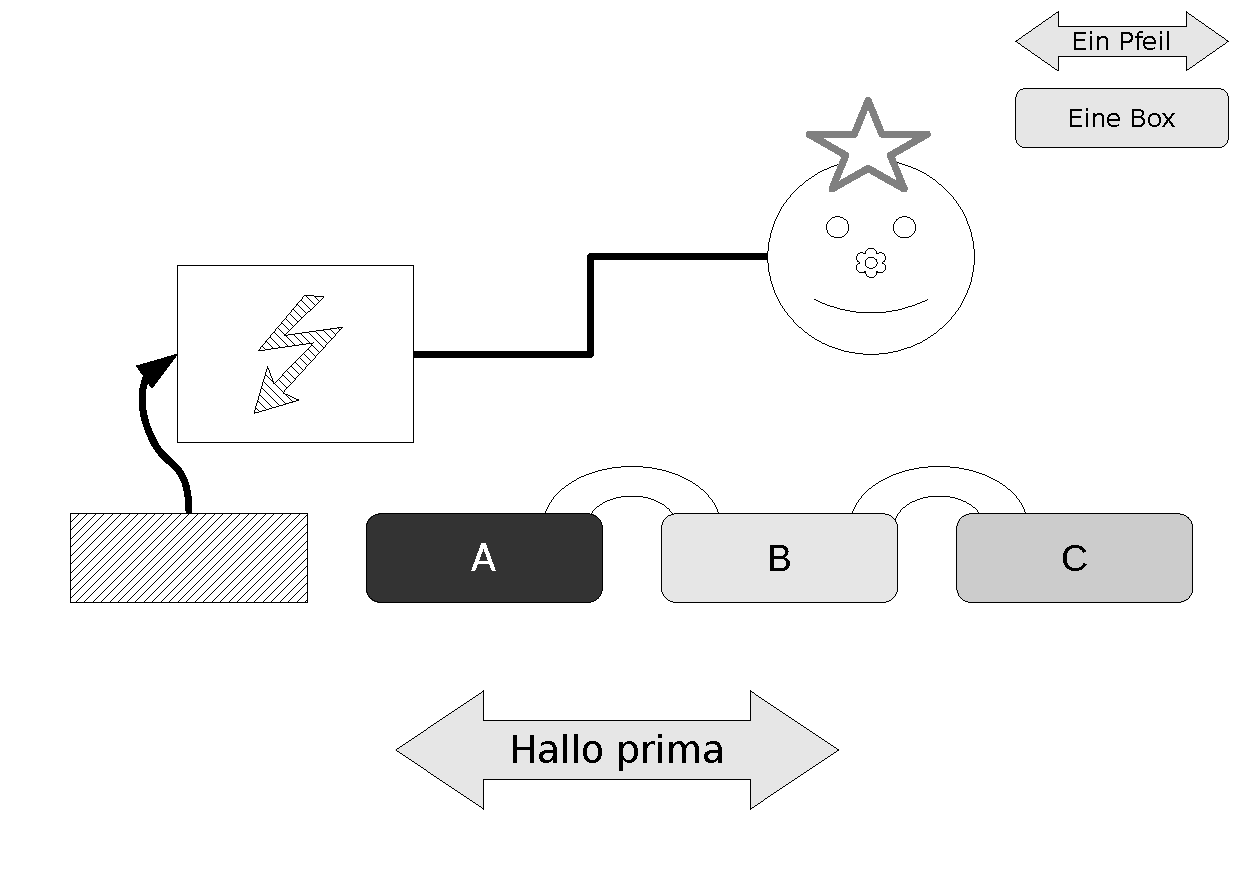
\includegraphics[width=.9\textwidth]{zeichnung.eps}
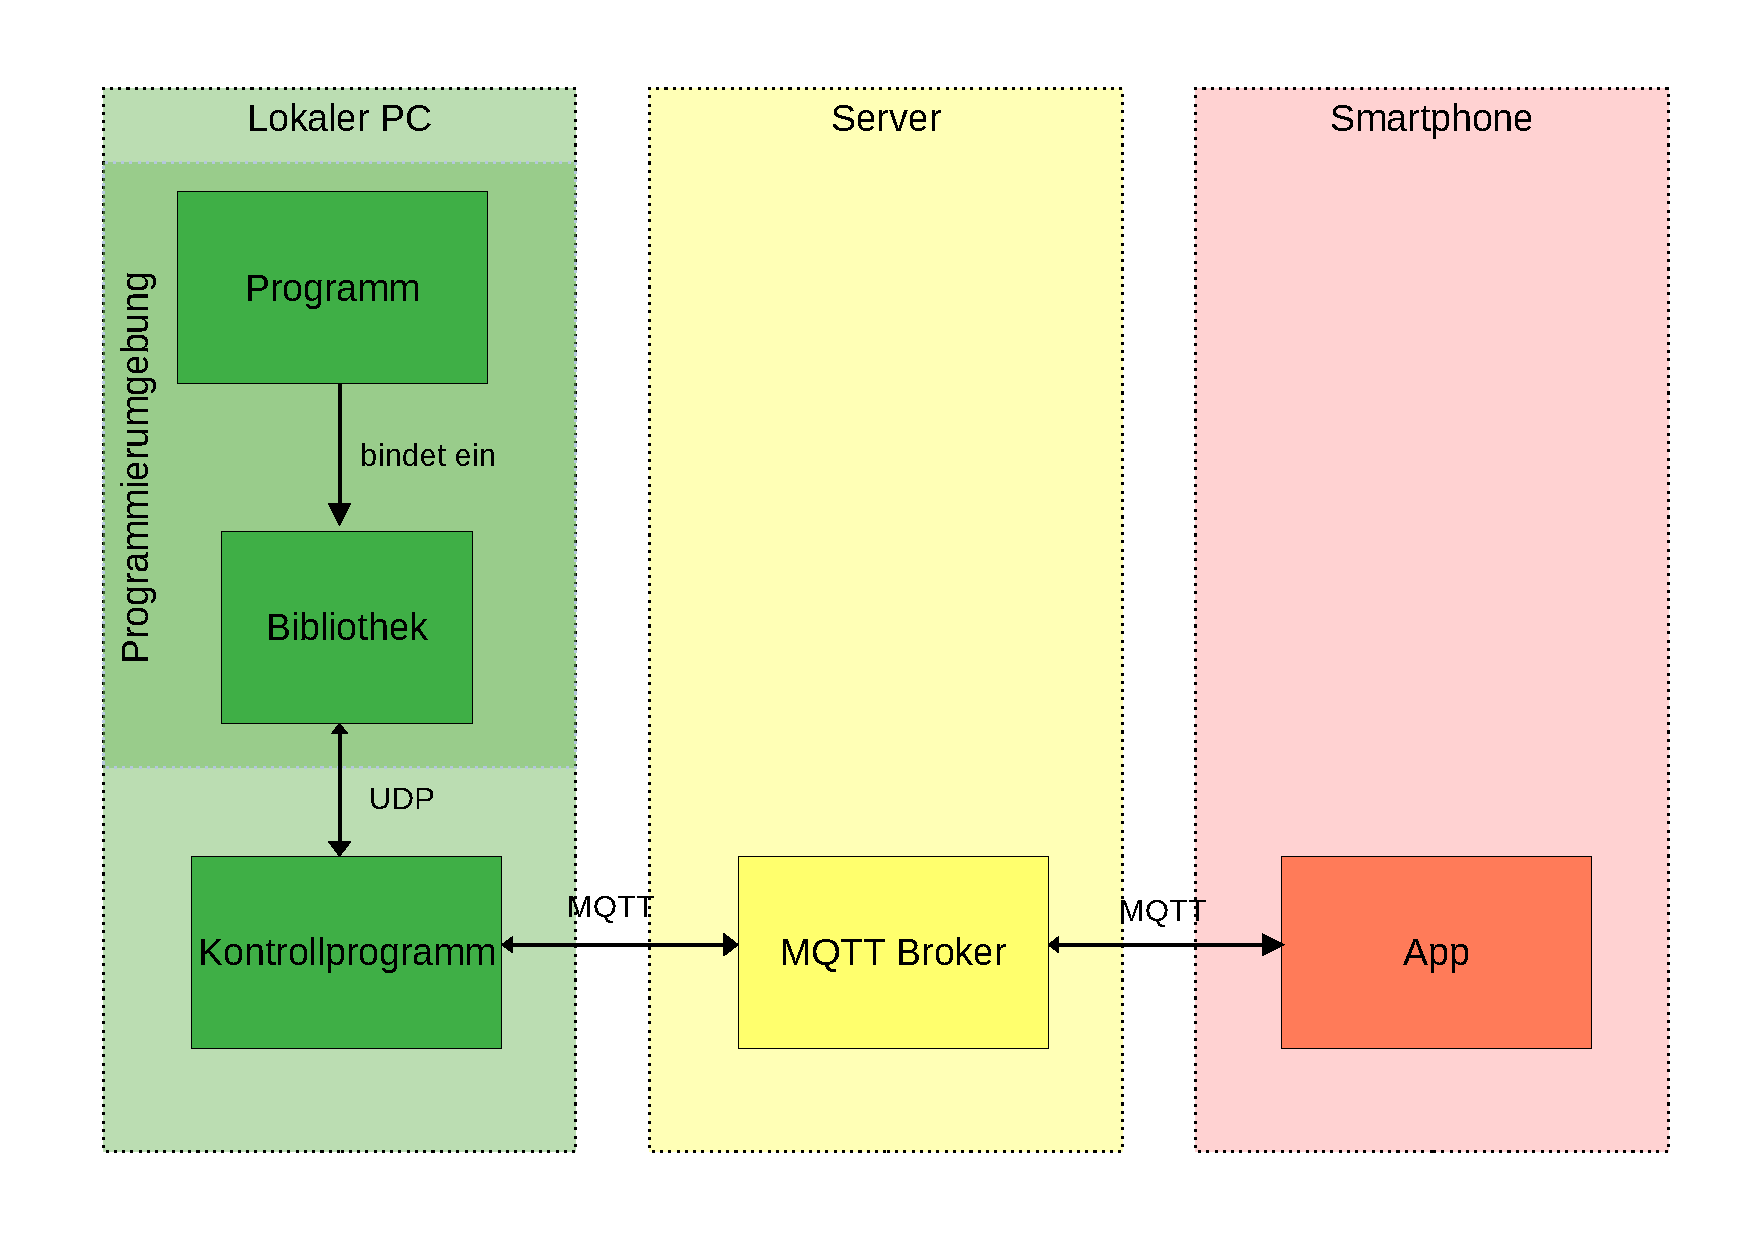
\includegraphics[width=\textwidth]{images/framework.pdf}
\caption{System-Aufbau}
\label{fig:design}
\end{figure}
Um mit dem Smartphone zu interargieren bietet die Programmierumgebung eine programmiersprachenunabhängige Bibliothek mit Schnittstellen in Form von Stub-Funktionen an, die die \acrshort{api} der Kontrollanwendung nutzen.
Die Bibliothek kann in bestehenden Programmcode zum Zweck der Nutzung eingebunden werden.
Zur Unterstützung der Verständlichkeit für angehende Programmierer wurde bei der Entwicklung der Bibliothek auf die Implementierung von Funktionen mit asynchronen Rückgabewerten, wie beispielsweise Futures, verzichtet.
Die in der Programmiersprache Python imlementierte Kontrollanwendung, welche ebenfalls auf dem lokalen PC betrieben wird, dient der Nachrichtenvermittlung zwischen Smartphone-App und Programmierumgebung.
%todo: das hier ist Prozess. Abtrennen?
Führt ein Programmierer einen Funktionsaufruf der Bibliothek aus, übermittelt die Bibliothek diesen per \acrshort{udp} dem Kontrollprogramm welches über die weitere Verfahrensweise entscheidet.
Bei einer Ausgabeanfrage wird die Nachricht beispielsweise per \acrshort{mqtt} an das Smartphone übertragen.
Die Kontrollanwendung speichert zudem Sensormesswerte unpersistent in einem Key-Value-Store um Sie zu cachen.
Zum Cachen werden Messwerte in regelmäßigen Abständen von der Smartphone-App an die Kontrollanwendung übermittelt.
Bei Eingang einer Sensorwert-Anfrage der Bibliothek sendet die Kontrollanwendung den zuletzt von der Smartphone-App übermittelten Wert an die Bibliothek zurück.
%todo: wo wird erwähnt in welcher Programmiersprache die App geschrieben ist?

Zur Übermittlung der Nachrichten werden die Protokolle MQTT und UDP eingesetzt.
MQTT ist ein auf einem Observer-Pattern basierendens Client-Server-Protokoll.
Durch einen 2 Byte großen Header und maximalen Payload-Größe von 260 MB ist es leichtgewichtig und gleichzeitig flexibel.
Nachrichten werden zur Publizierung auf einem Topic an einen MQTT Broker gesendet.
Dieser leitet sie dann an alle Clients weiter die das Topic abboniert haben.
%todo: MQTT Nutzung wurde vom Prof vorausgesetz reinbringen.
Die UDP-Kommunikation zwischen Bibliothek und Kontrollprogramm auf dem lokalen PC wird über ein Loopback-Interface umgesetzt um die Latenzzeiten zwischen Programmierumgebung und Kontrollprogramm zu minimieren.
Als Nachrichtenformat wird \acrshort{json} verwendet.
Das menschlesbare, kompakte Nachrichtenformat ist weit verbreitet und wird von vielen Softwarebibliotheken unterstützt.

\chapter{Nachrichtenformate}\label{chap:message_formats}
Ein einheitliches Nachrichtenformat ist Voraussetzung für den Nachrichtenaustausch.
Der ausgearbeitete Nachrichtenstandard definiert die Nachrichten in einem Klartextformat.
Nachrichten-Vorlagen sind in einer Datei gespeichert und werden in der Bibliothek, dem Kontrollprogramm und in der Smartphone-App eingelesen, wodurch Sie in allen Komponenten kongruent vorliegen.
Es gibt unterschiedliche Nachrichtentypen, welche in Tabelle \ref{tab:message_types} aufgeführt sind.
Zur besseren Nachvollziehbarkeit der Kommunikation sind außerdem Quelle, Ziel und das verwendete Netzwerkprotokoll angegeben.
Eine Liste der vollständigen Nachrichtentypen, inklusive ihrer Felder, ist im Anhang aufgeführt.
\begin{table}[htbp]
  \centering
  \begin{tabular}{|l|p{30mm}|c|c|}
      \hline
      \textbf{Nachrichtentyp} & \textbf{Quelle} & \textbf{Ziel} & \textbf{Netzwerkprotokoll}\\
      \hline
		sensor\_request & Bibliothek & Kontrollprogramm & UDP\\
       \hline
       sensor\_response & Kontrollprogramm & Bibliothek & UDP\\
       \hline
		update\_request & Smartphone & Kontrollprogramm & MQTT\\
       \hline
		rpc\_request & Bibliothek, Kontrollprogramm & Smartphone & UDP/MQTT\\
       \hline
		rpc\_response & Smartphone, Kontrollprogramm & Bibliothek & UDP/MQTT\\ 
       \hline
  \end{tabular}
  \caption{Nachrichten-Typen}
  \label{tab:message_types}
\end{table}

\textit{Sensor\_request}s kommen bei Sensormesswert-Abfragen zum Einsatz.
%todo: zwischengespeichert hat hört sich kacke an. 
Dieser Nachrichttyp wird von der Bibliothek an das Kontrollprogramm gesendet, wo die vom Smartphone übermittelten Sensorwerte zwischengespeichert wurden.
Nach Eingang ermittelt das Kontrollprogramm, durch Angabe des gewünschten Sensortyp-Kürzels im Feld \texttt{sensor\_type}, den gespeicherten Sensormesswert.
Sensortyp-Kürzel sind für alle Sensoren definiert und dienen in der Kontrollanwendung als Schlüssel der Addressierung der Messwerte im Key-Value-Speicher.
Die Kürzel sind in Tabelle \ref{tab:sensor_types} aufgelistet. 
\begin{table}[htbp]
  \centering
  \begin{tabular}{|c|c|}
      \hline
      \textbf{TYPE-Kürzel} & \textbf{Beschreibung} \\
      \hline
      accel\_\{x,y,z\} & Lagesensor für die X, Y oder Z-Richtung \\
      \hline
       gyro\_\{x,y,z\} & Gyroskopsensor für die X, Y oder Z-Richtung \\
      \hline
      prox & Näherungssensor \\
      \hline
  \end{tabular}
  \caption{Sensor-Kürzel mit Beschreibung}
  \label{tab:sensor_types}
\end{table}
Ist für den Sensortyp ein Sensormesswert im Key-Value-Store vorhanden, wird das Ergebnis in einer \textit{sensor\_response}, im Feld \texttt{sensor\_value}, zurückgesendet.
Die Antwort wird von der Bibliothek angenommen und an die aufrufende Funktion zurückgegeben.
Um stets aktuelle Sensormesswerte zu erhalten, müssen sie vom Smartphone in regelmäßigen Zeitabständen übermittelt werden.
Die Android-App sendet daher in periodischen Abständen Nachrichten des Typs \textit{update\_request} an das Kontrollprogramm.
Übermittelt werden zur Einspeicherung und Zuordnung im Key-Value-Store sowohl der Sensortyp als auch der Sensormesswert.
Der gesamte Ablauf der Sensordatenübertratung ist in Abbildung \ref{fig:message_flow_requests} dargestellt.
\begin{figure}[htbp]
\centering
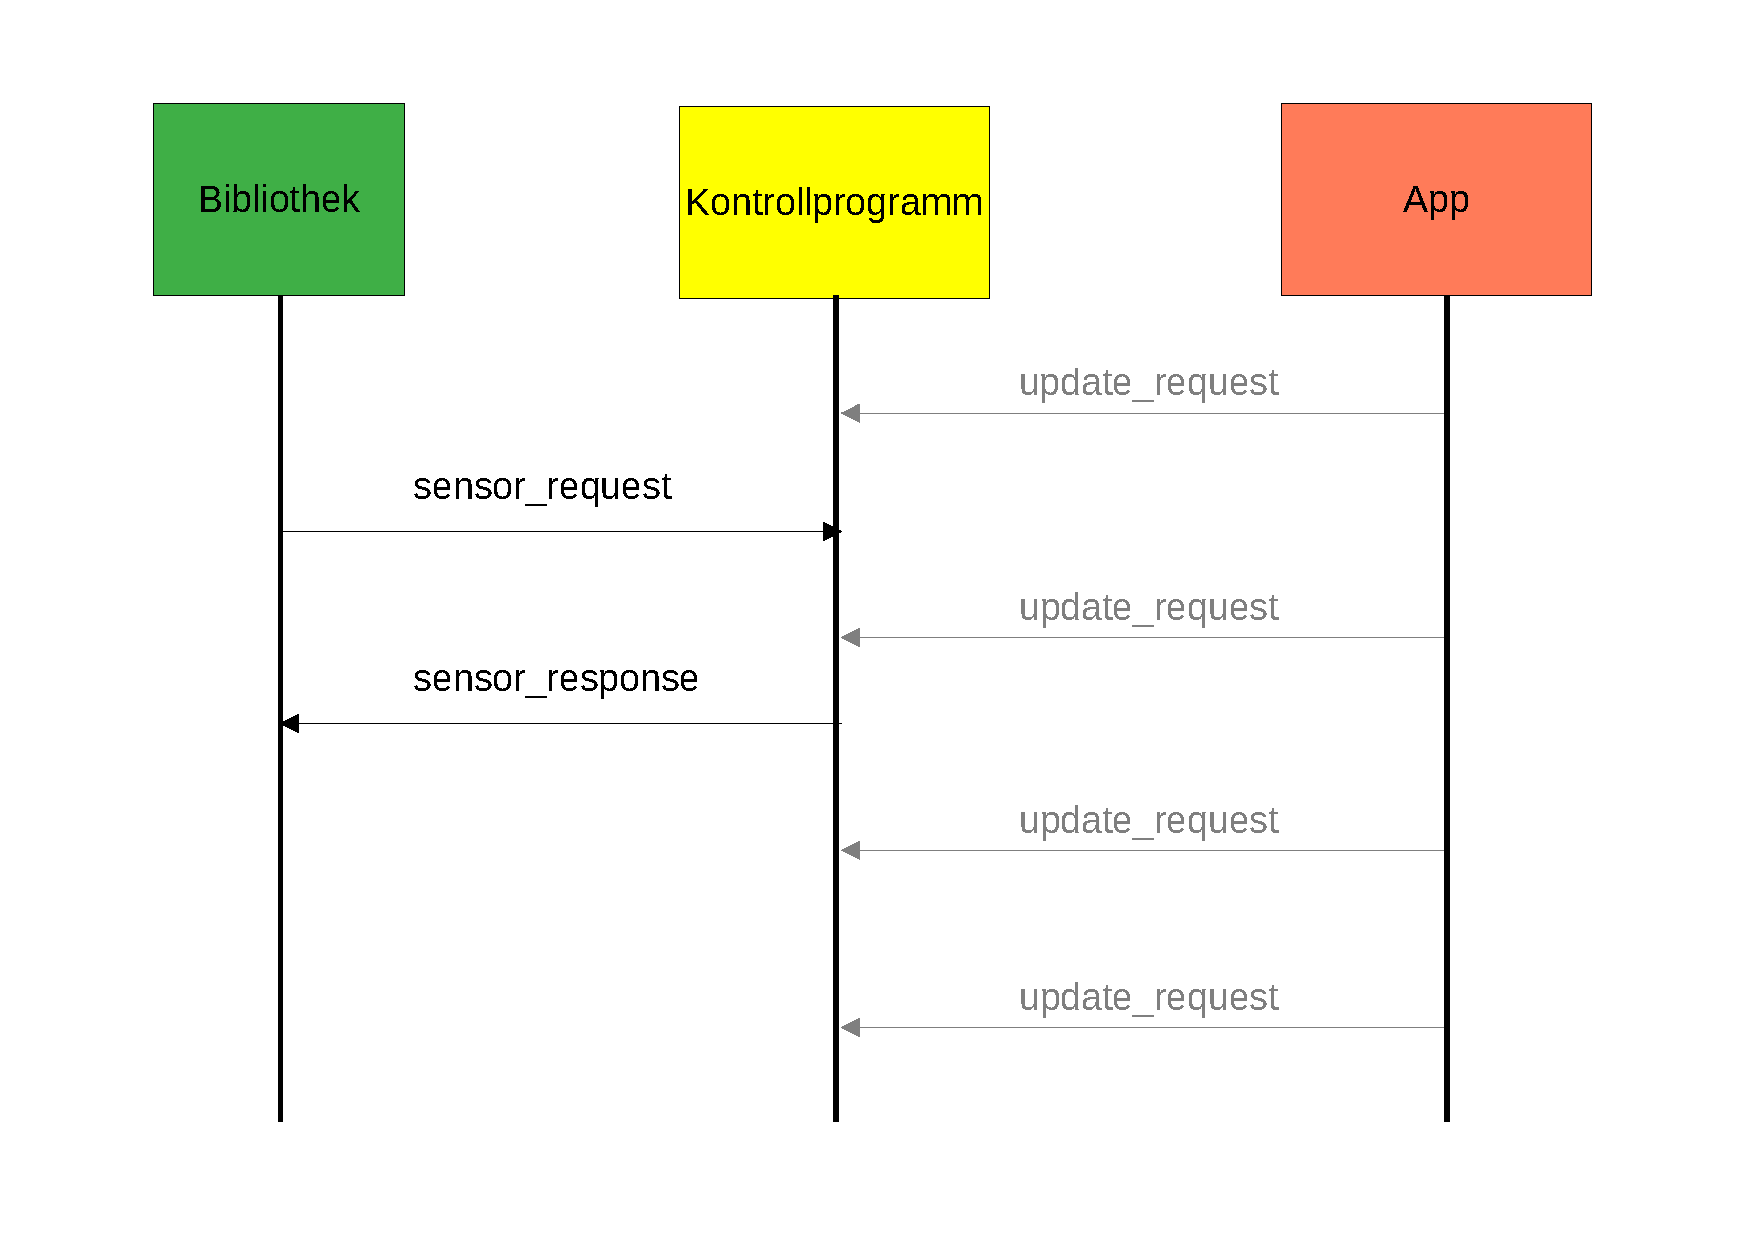
\includegraphics[width=.6\textwidth]{images/message_flow_sensor}
\caption{Nachrichtenablauf der Sensordatenübermittlung}
\label{fig:message_flow_requests}
\end{figure}
Aufgeführt sind die drei Komponenten Bibliothek, Kontrollprogramm und Smartphone-App.
Die Bibliothek sendet sensor\_requests per UDP an das Kontrollprogramm.
Dieses antwortet über UDP mit einer sensor\_response.
Währenddessen werden der Kontrollanwendung vom Smartphone fortwährend neue Sensormesswerte durch update\_requests übertragen.

Neben Nachrichten die die Sensordatenübermittlung betreffen, existieren zur Umsetzung von Ausgaben auf der Smartphone-App auch Ausgabe-Nachrichten.
Die Appseitigen Ausgaben sind unterscheidbar in Ausgaben mit und ohne Rückgabewert.
Für erstere gibt es den Nachrichtentyp \textit{rpc\_request}.

\acrshort{rpc} (Remote Procedure Call) und bezeichnet clientseitige Funktionsaufrufe, die auf einem Server ausgeführt werden.
Die Bezeichnung entspricht nicht exakt dem Konzept, da ein Kommunikationspartner, Smartphone-App oder Kontrollanwendung, in diesem Fall die Rolle des Servers einnehmen würde.
Die Voraussetzung einer Client-Server-Anwendung ist durch die beidseitige Nachrichtenübertragung zwischen Smartphone-App und Kontrollanwendung nicht gegeben.
Die Bezeichnung wurde unter dem Fokus auf der entfernten Ausführung einer Funktion gewählt und entspricht eher einer Remote Method Invocation (\acrshort{rmi}).

Der Nachrichtentyp rpc\_request enthält die Felder \texttt{command} und \texttt{value}.
Diese spezifizieren die Ausgabe und falls vorgesehen eine mit der Ausgabe verbundene Größe.
Für die Vibrationsausgabe wären die Inhalte des rpc\_requests für eine Vibration von einer Sekunde beispielsweise \textit{vibrate} und \textit{1000}.
Die Nachricht wird von der Bibliothek per UDP an die Kontrollanwendung und von dort aus per MQTT an das Smartphone gesendet.
Die Smartphone-App nimmt die Anfrage an und führt die Ausgabe aus.
Manche Ausgabe-Anweisungen geben zusätzlich einen Rückgabewert zurück.
Damit dieser vom Smartphone zurück an die Bibliothek gesendet werden kann, gibt es das Nachrichtenformat \textit{rpc\_response}.
Eine Nachricht dieser Nachrichtenart wird erst per MQTT an das Kontrollprogramm und von dort aus per UDP an die Bibliothek gesendet.
Der Nachrichtenablauf wird in Abbildung \ref{fig:message_flow_rpc} dargestellt.
\begin{figure}[htbp]
\centering
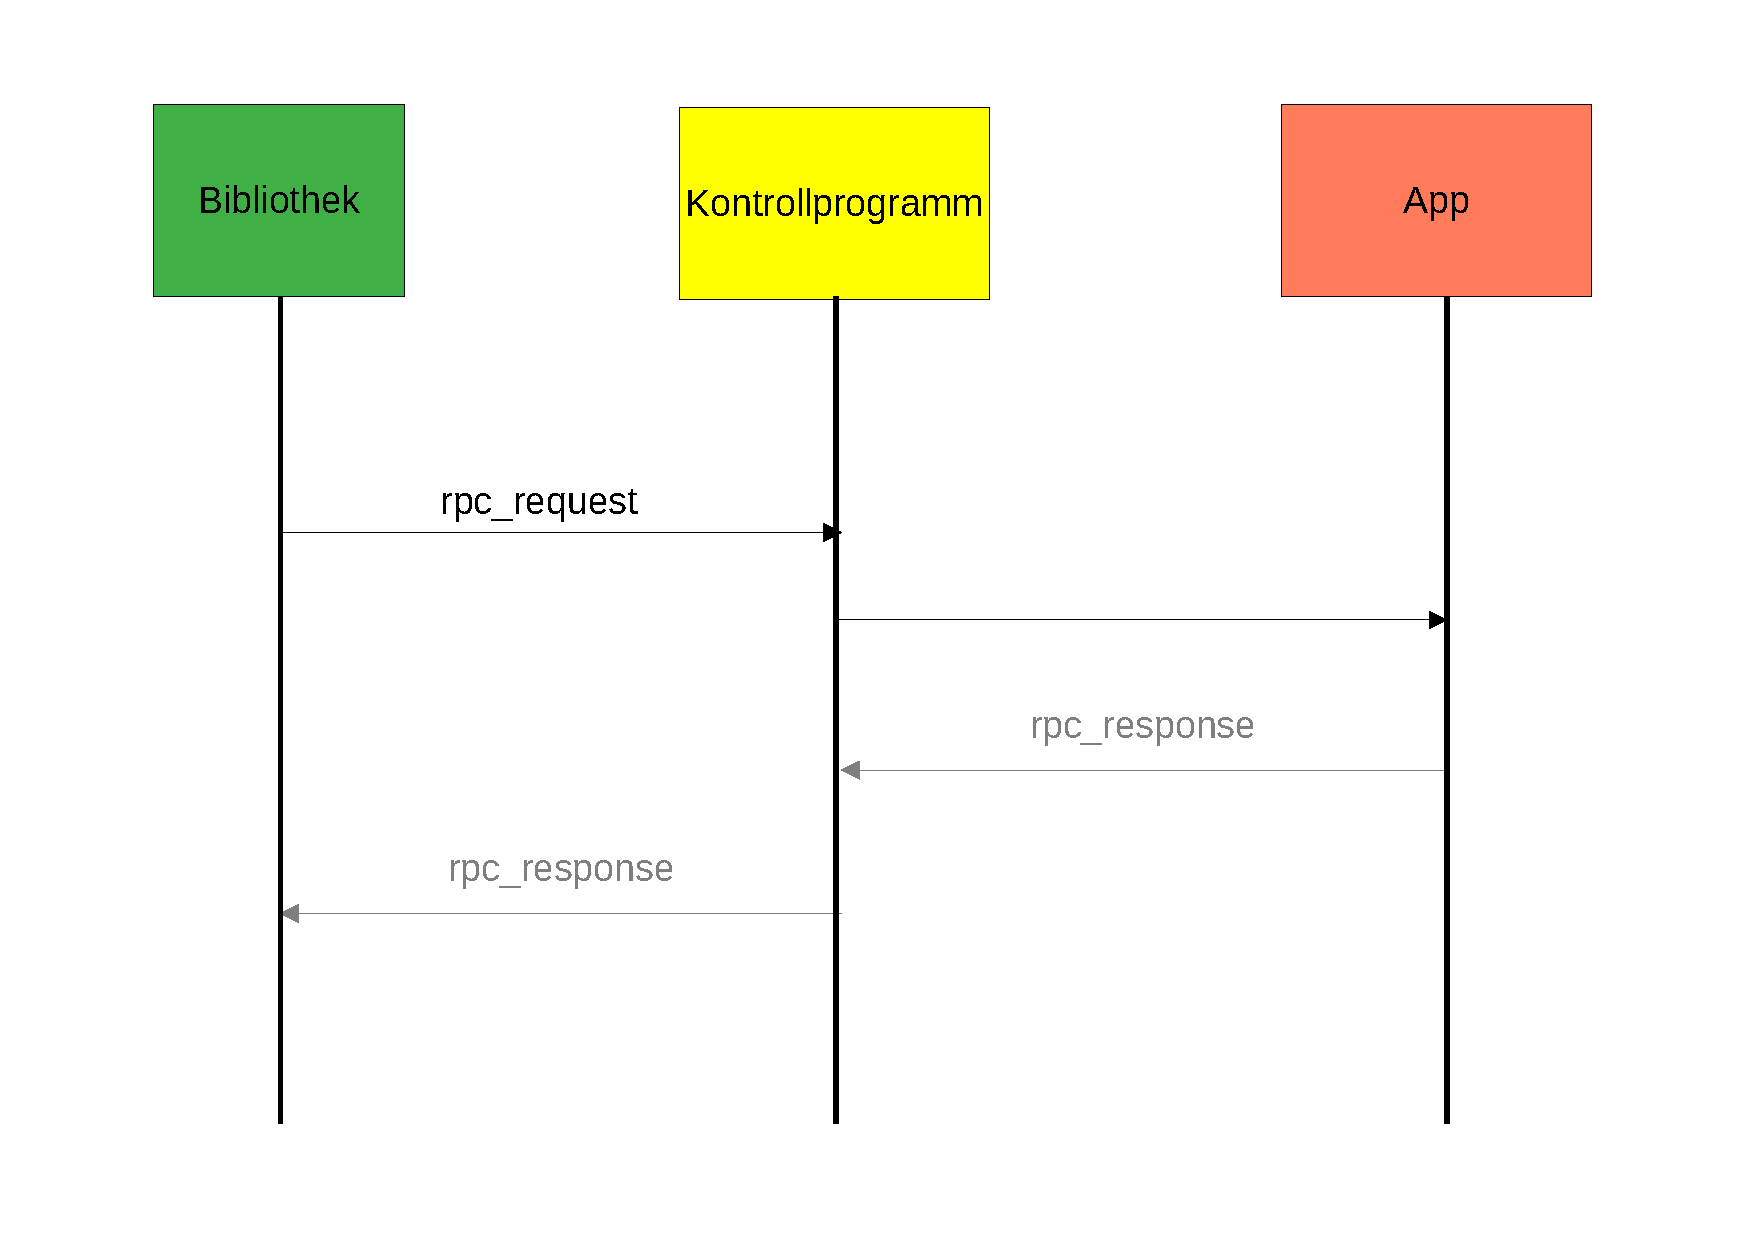
\includegraphics[width=.6\textwidth]{images/message_flow_rpc.pdf}
\caption{Nachrichtenablauf der RPC-Anfragen}
\label{fig:message_flow_rpc}
\end{figure}
Aufgeführt sind die drei Komponenten Bibliothek, Kontrollprogramm und Android-App.
Die Bibliothek sendet ein rpc\_request per UDP an das Kontrollprogramm.
Dieses leitet die Nachricht per MQTT weiter an die Smartphone-App, wo das Kommando ausgeführt wird.
Ein eventuell anfallender Rückgabewert wird durch eine rpc\_response vom Smartphone per MQTT zurück an die Kontrollanwendung gesendet, welche die Nachricht dann per UDP weiter an die Bibliothek weiterleitet.


\chapter{Android Anwendung}\label{chap:app}
Die Android-Anwendung ist eine der drei Bestandteile des Frameworks.
Sie dient dazu Sensormessprozesse zu starten, Sensordaten zu übermitteln und Ausgabe-Kommandos auszuführen.
Für diese bietet Sie eine Signal-LED, ein Textfeld und zwei Buttons in einer RootActivity an.
Neben UI-Elementen gibt es zusätzlich noch eine Vibrationsausgabe. 
Die Anwendung initiiert zum Start Sensormessprozesse und sendet unter Verwendung von SensorEventListenern die Sensormessdaten in periodischen Zeitabständen an die Kontrollanwendung.
Verwendete Sensoren sind beispielsweise der Lagesensor oder das Gyroskop des Smartphones.
Die gemessenen Werte werden über einen im Hintergrund ausgeführten MQTT-Service versandt, welcher ebenfalls auf eingehende Nachrichten reagiert, um Ausgaben auf dem Smartphone auszulösen.

\section{Startvorgang}
Ein Ablaufplan des Startvorgangs ist in Abbildung \ref{fig:app_flow} zu sehen.
%Todo: Hier fehlen noch die Schritte der EInbindung und Gedöns das ursprünglich nicht rein solte
\begin{figure}[htbp]
  \centering
  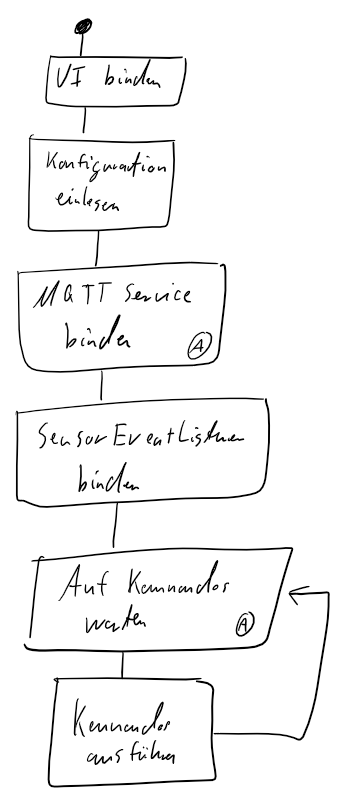
\includegraphics[width=0.8\textwidth]{images/app_ablauf}
  \caption{Ablaufdiagramm Android Anwendung}
  \label{fig:app_flow}
\end{figure}
In der RootActivity werden anfänglich alle UI-Elemente zur programmatischen Ansteuerung eingebunden.
Anschließend werden die zwei Konfigurationsdaten config.json und protocol.json eingelesen.
In Ersterer sind grundlegende Konfigurationsparameter wie Hostname und Port des MQTT-Brokers oder der Name des Topics definiert.
In der Datei protocol.json werden neben den Schlüsselwörtern und Abkürzungen für Sensortypen und Ausgabekommandos auch Vorlagen für Nachrichtenformate aufgeführt.

Nach dem Einlesen der Konfigurationen wird der zur Kommunikation verwendete MQTT-Service gestartet und asynchron eingebunden.
Über eine ServiceConnection wird beim erfolgreichen Einbinden über eine Callback-Methode der weitere Ablauf der Anwendung definiert, der erst ausgeführt werden soll, wenn eine MQTT-Verbindung hergestellt ist.
RootActivity und MQTT-Service tauschen jeweils ihre Objekt-Referenzen aus.
Methoden des MQTT-Service rufen zum Zweck der Ausgabe Methoden der RootActivity auf.
SensorEventListener benötigen eine Referenz auf den MQTT-Service, da sie bei Sensorwerten über diesen update\_requests versenden.

Der Nachrichtenempfang im MQTT-Service wird nicht im UI-Thread behandelt.
Dies ist jedoch Voraussetzung um UI-Elemente wie die Signal-LED im Service verändern zu können.
Android unterbindet Änderungen der UI-Elemente wenn der verändernde Thread nicht der UI-Thread ist.
Dieses Problem wird durch die Methode \textit{runOnUiThread} umgangen, welche die Änderung in der Ausführungswarteschlange des UI-Threads einreiht.

Der MQTT-Service baut eine Verbindung zu einem in Datei config.json definierten MQTT-Broker auf und abboniert ein ebenfalls in der Konfigurationsdatei angegebenes Topic.
Ist der MQTT-Service eingebunden sind alle Voraussetzungen für eine Übertragung erfüllt und  Sensormessprozesse können gestartet werden.
Die Funktionsweise der Sensormeessung wird in Abbildung \ref{fig:sensor_event_listener} dargestellt.
\begin{figure}[htbp]
  \centering
  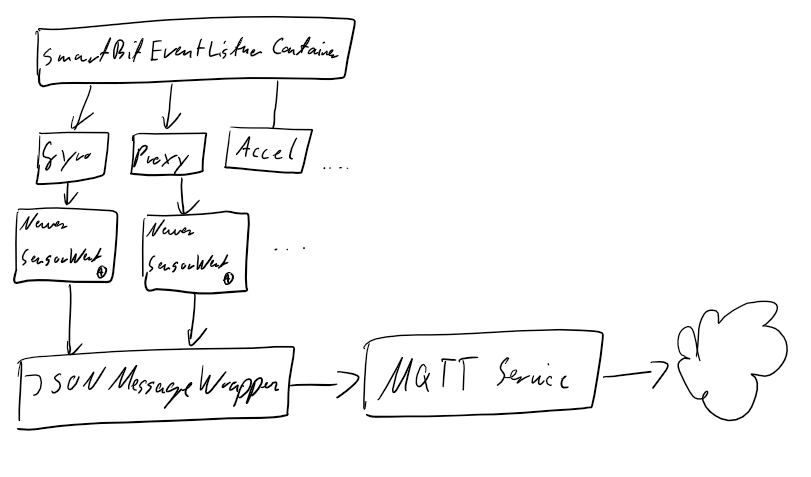
\includegraphics[width=.8\textwidth]{images/sensor_event_listener.png}
  \caption{Ablauf SensorEventListener}
  \label{fig:sensor_event_listener}
\end{figure}
SensorEventListener werden, nach Prüfung der Verfügbarkeit der jeweiligen Sensoren, gestartet und zentral in einem \texttt{SmartBitEventListenerContainer} gespeichert.
Diese Klasse beeinhaltet SensorEventListener für alle untertstützten Sensoren und dient der Datenhaltung der einzelnen SensorEventListener.
Aufgabe der SensorEventListener ist es auf Sensorwert-Änderungen zu reagieren und eine entsprechende Callback-Funktion in der die Sensorwerte über den MQTT-Service per update\_requests an die Kontrollanwendung übermittelt werden.
Statische Methoden der Klasse \textit{JSONMessageWrapper} ermöglichen die Erstellung der Nachrichtenformate und setzen das Messergebniss in das korrekte Feld ein.
Die so generierte Nachricht wird anschließend über den gebundenen MQTT-Service an das vorher definierte Topic versendet.

Anschließend ist die Startroutine der Mobilen Anwendung abgeschlossen.
Auf Nachrichten wird nun nur noch im MQTT-Service in einem MessageListener mit entsprechendem Callback reagiert und gegebenenfalls eine Ausgabe ausgeführt.
Die Anwendung ist nun betriebsbereit und sendet update\_requests an die Kontrollanwendung.
Übermittelt werden die Sensordaten an den Broker mit einer \acrshort{qos}-Stufe von 0.
Auf dieser Stufe wird der Empfang der Nachricht von den Kommunikationspartnern nicht bestätigt.
Verluste von update\_requests sind unproblematisch, da je nach Taktung der SensorEventListener innerhalb kurzer Zeit neue Sensormesswerte zur Übertragung vorliegen.
Eine exakte Zustellung ist hier nicht notwendig.
Höhere QoS-Stufen würden den Übertraungsprozess verlangsamen und Latenzen erhöhen.

\section{Sensoren}
Smartphones beeinhalten Sensoren, die Daten über die Umgebungseigenschaften erfassen.
Dazu zählen Beispielsweise Bewegung, Annäherung, aber auch Temperatur oder Luftdruck.
%todo: stimmt nicht. die messen einfach. reagiert wird wo anders.
Ihr Zweck besteht darin auf Änderungen der Werte zu reagieren.
Für unterschiedliche Aufgaben werden unterschiedliche Sensoren benötigt.
Beispielsweise word für \textit{Diebstahl-Alarm} nur der Näherungssensor verwendet, für \textit{Dreh-Zähler} der Lagesensor.
Insgesamt werden in der Android Anwendung werden folgende Sensortypen verwendet: Lineare Beschleunigungssensoren, Gyroskop und Annäherungssensor.

Beschleunigungs- bzw. Lagesensoren messen die Beschleunigung in $m/s^2$ für die drei Bewegungsrichtungen: X-, Y- und Z-Achse in einem festgelegten Zeitraum.
Die Erdbeschleunigung ist auch in diesen Messwerten enthalten.
Diese muss für die bereinigten, realen Werte von den aufgenommenen Werten subtrahiert werden\cite{accel_g}.
% todo: einheiten
Messeinheiten unterscheiden sich je nach Sensor.
Das Gyroskop misst keine Beschleunigung sondern die aktuelle Geschwindigkeit in $rad/s$ der gleichen Achsen.
Zur Übersicht sind diese in Abbildung \ref{fig:and_axes} zu dargestellt.
\begin{figure}[htbp]
  \centering
  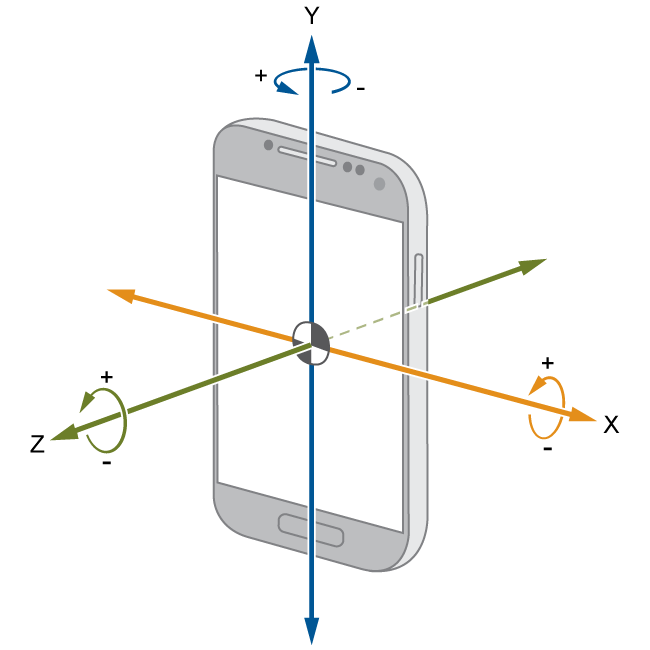
\includegraphics[width=.7\textwidth]{images/android_axes.png}
  \caption{Android-Koordinatensystem}
  \label{fig:and_axes}
\end{figure}
Die Frequenz mit der Messwerte erfasst werden kann manuell angegeben werden.
Hierfür stehen vier Stufen zur Auswahl.
\begin{table}[htbp]
  \centering
  \begin{tabular}{|c|p{4cm}|}
      \hline
      \textbf{Bezeichnung} & \textbf{Verzögerung} \\
	  \hline
      SENSOR\_DELAY\_FASTEST & Keine. Verwendet die Frequenz des Sensors.\\
      \hline
      SENSOR\_DELAY\_GAME & 20 ms\\
      \hline
      SENSOR\_DELAY\_UI & 60 ms\\
      \hline
      SENSOR\_DELAY\_NORMAL & 200 ms\\
      \hline
  \end{tabular}
  \caption{Sensor-Taktgeschwindigkeiten\cite{sensor-takt}}
  \label{tab:sensor_speeds}
\end{table}
In der Android-App erfolgen alle Messungen mit SENSOR\_DELAY\_NORMAL.
Die Stufe gilt für Android jedoch nicht als festes Limit, sondern wird eher als Richt-Frequenz behandelt.
Android kann die reale Frequenz auch erhöhen.
Nicht alle Smartphones besitzen alle Sensoren.
Daher wird beim Start überprüft ob der Sensor auch wirklich vorhanden ist.
Ist er es nicht, wird auch keine Messung gestartet.

\chapter{Kontrollanwendung}\label{chap:server_software}
%todo: se chapter needs some more sciency lingu
Zur Vermittlung zwischen den Komponenten fungiert als Middleware eine Kontrollanwendung.
Sie ist in Python geschrieben und vermittelt zwischen UDP-Anfragen auf der einen Seite vom Client aus und MQTT-Anfragen vom Smartphone auf der anderen Seite.
User können über die Library RPC-Anfragen oder Sensor-Anfragen an den Server stellen.
Dies geschieht in Form von JSON-Anfragen die per UDP übermittelt werden.
Der Server ist unter der localhost-Adresse 127.0.0.1 auf dem Port 5006 erreichbar.
Für die MQTT-Verbindung kommt dabei die unter OpenSource-Liznenz stehende MQTT-Library Paho \cite{paho} der Eclipse-Foundation zum Einsatz. 

Die Kontrollanwendung ist aufgeteilt in einen Datenverwaltungsteil, DataHandler, und eine MQTT Anbindung, MQTTHandlerThread.
Der zur Sensordatenpufferung dienende Key-Value-Store wird durch die Klasse SensorDB implementiert.
Diese Wrapper-Klasse bietet threadsichere Zufriffsfunktionen auf ein intern gespeichertes Python-Dictionary.
Eine Übersicht über die Komponenten der Kontrollanwendung ist in Abbildung \ref{fig:serverUml} dargestellt.
\begin{figure}[htbp]
  \centering
  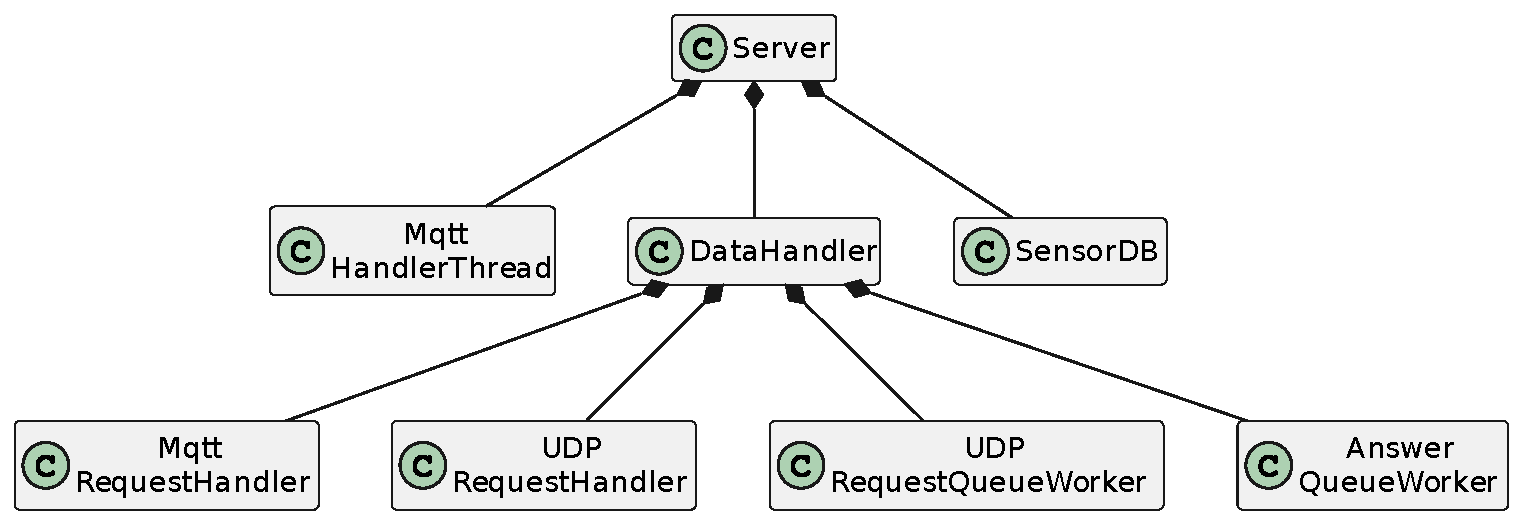
\includegraphics[width=\textwidth]{images/ServerUml}
  \caption{UML Digaramm Server}
  \label{fig:serverUml}
\end{figure}
DataHandler wiederrum teilt sich nochmal auf in vier seperate Funktionen, die als Threads nebenläufig laufen: MqttRequestHandler, UDPRequestHandler, UDPRequestQueueWorker und AnswerQueueWorker.

Die Funktionsweise und Zwecke dieser Threads wird im Folgenden an zwei Beispielen erläutert.
Für das erste Beispiel wird Abbildung \ref{fig:serverMqttReqPath} betrachtet.
\begin{figure}[htbp]
  \centering
  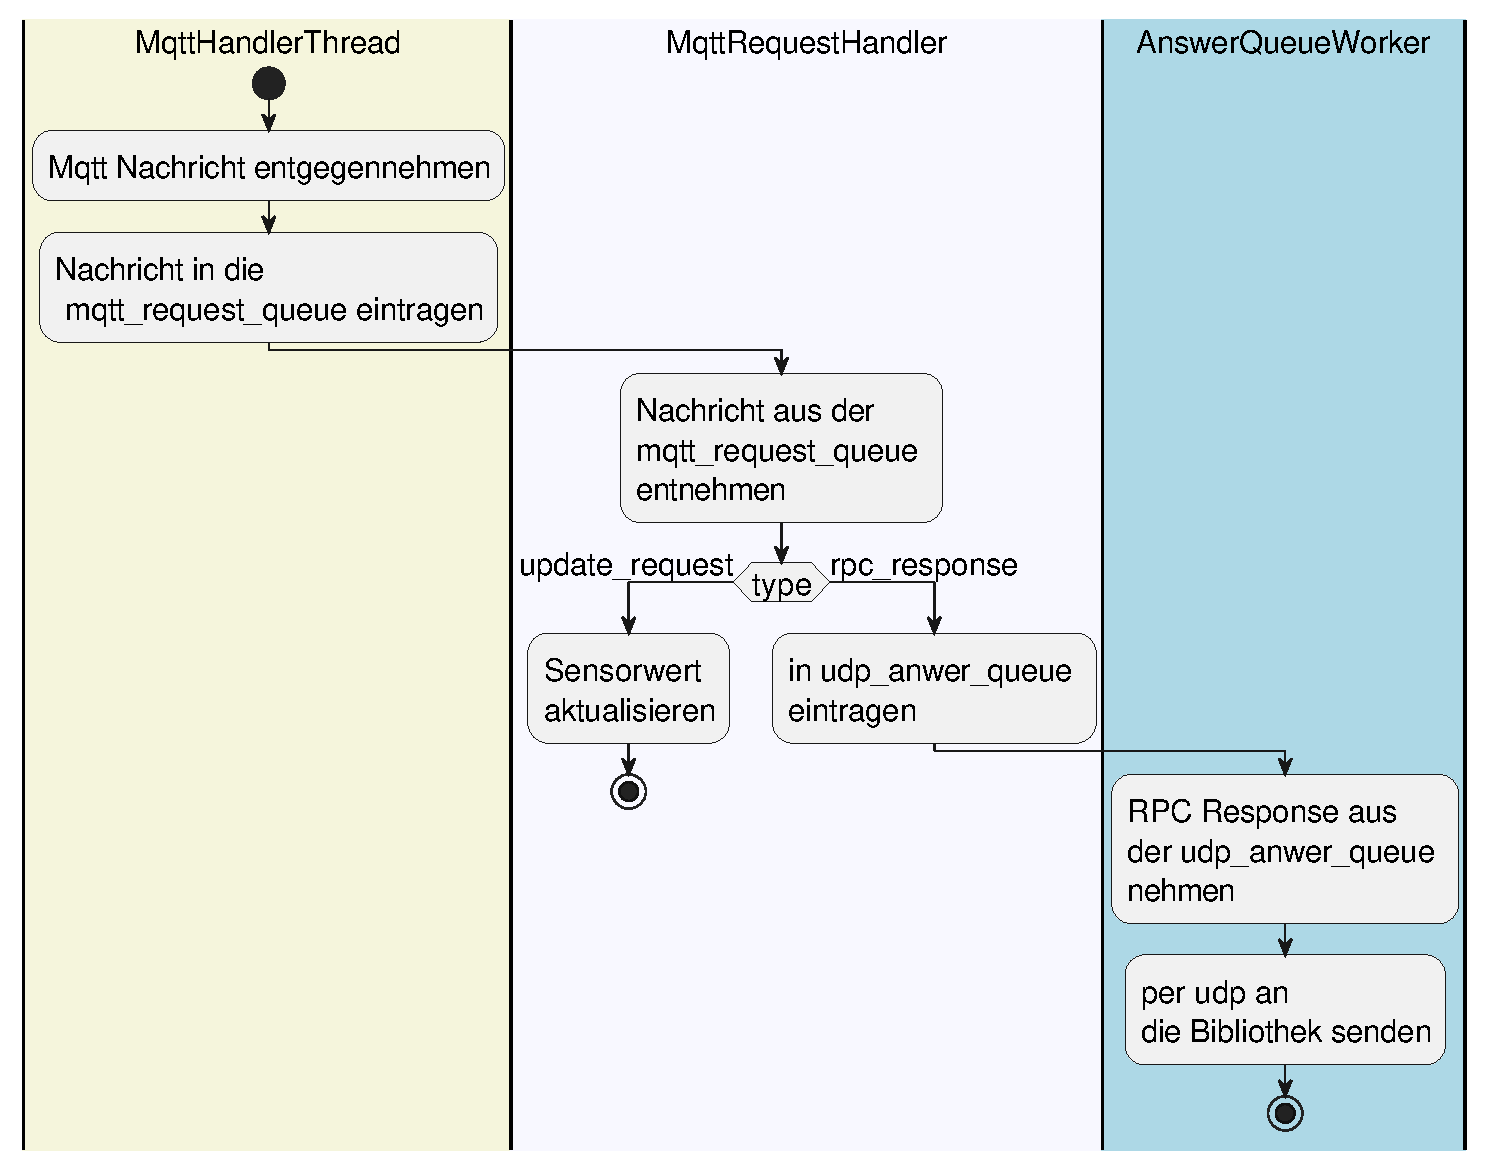
\includegraphics[width=\textwidth]{images/MqttRequestServerPath}
  \caption{Ablaufdiagramm MQTT Request}
  \label{fig:serverMqttReqPath}
\end{figure}
Dargestellt ist ein MQTT-Request, also eine Anfrage des Smartphones, dass über MQTT an den Server gesendet wird.
Erreicht ein MQTT Request den Server wird es im MQTTHandlerThread entgegengenommen.
Dieser setzt die Nachricht in eine MQTTRequestQueue ein.
Der MQTTRequestHandler des DataHandlers wartet bis ein Eintrag in der Queue vorhanden ist und nimmt gegebenenfalls eine Nachricht.
Daraufhin wird derTyp des Requests bestimmt.
Handelt sich um ein Sensorupdate muss nur der Sensorwert in der Datenbank aktualisiert werden.
Handelt es sich um eine rpc\_response, also um eine Antwort auf eine vorausgegangenes rpc\_request, dass einen Rückgabewert fordert, wird das request in eine udp\_answer\_queue eingefügt.
Der AnswerQueue Worker wartet, ähnlich wie der MQTT Request Handler, bis eine neue Nachricht vorhanden ist die per UDP an den Client gesendet werden soll und sendet diese dann gegebenfalls ab.

Das zweite Beispiel befasst sich mit dem Ablauf eines UDP-Requests, also einer Anfrage die mithilfe der Bibliothek gesendet wurde.
Der Ablauf ist in Abbildung \ref{fig:serverUDPReqPath} dargestellt.
\begin{figure}[htbp]
  \centering
  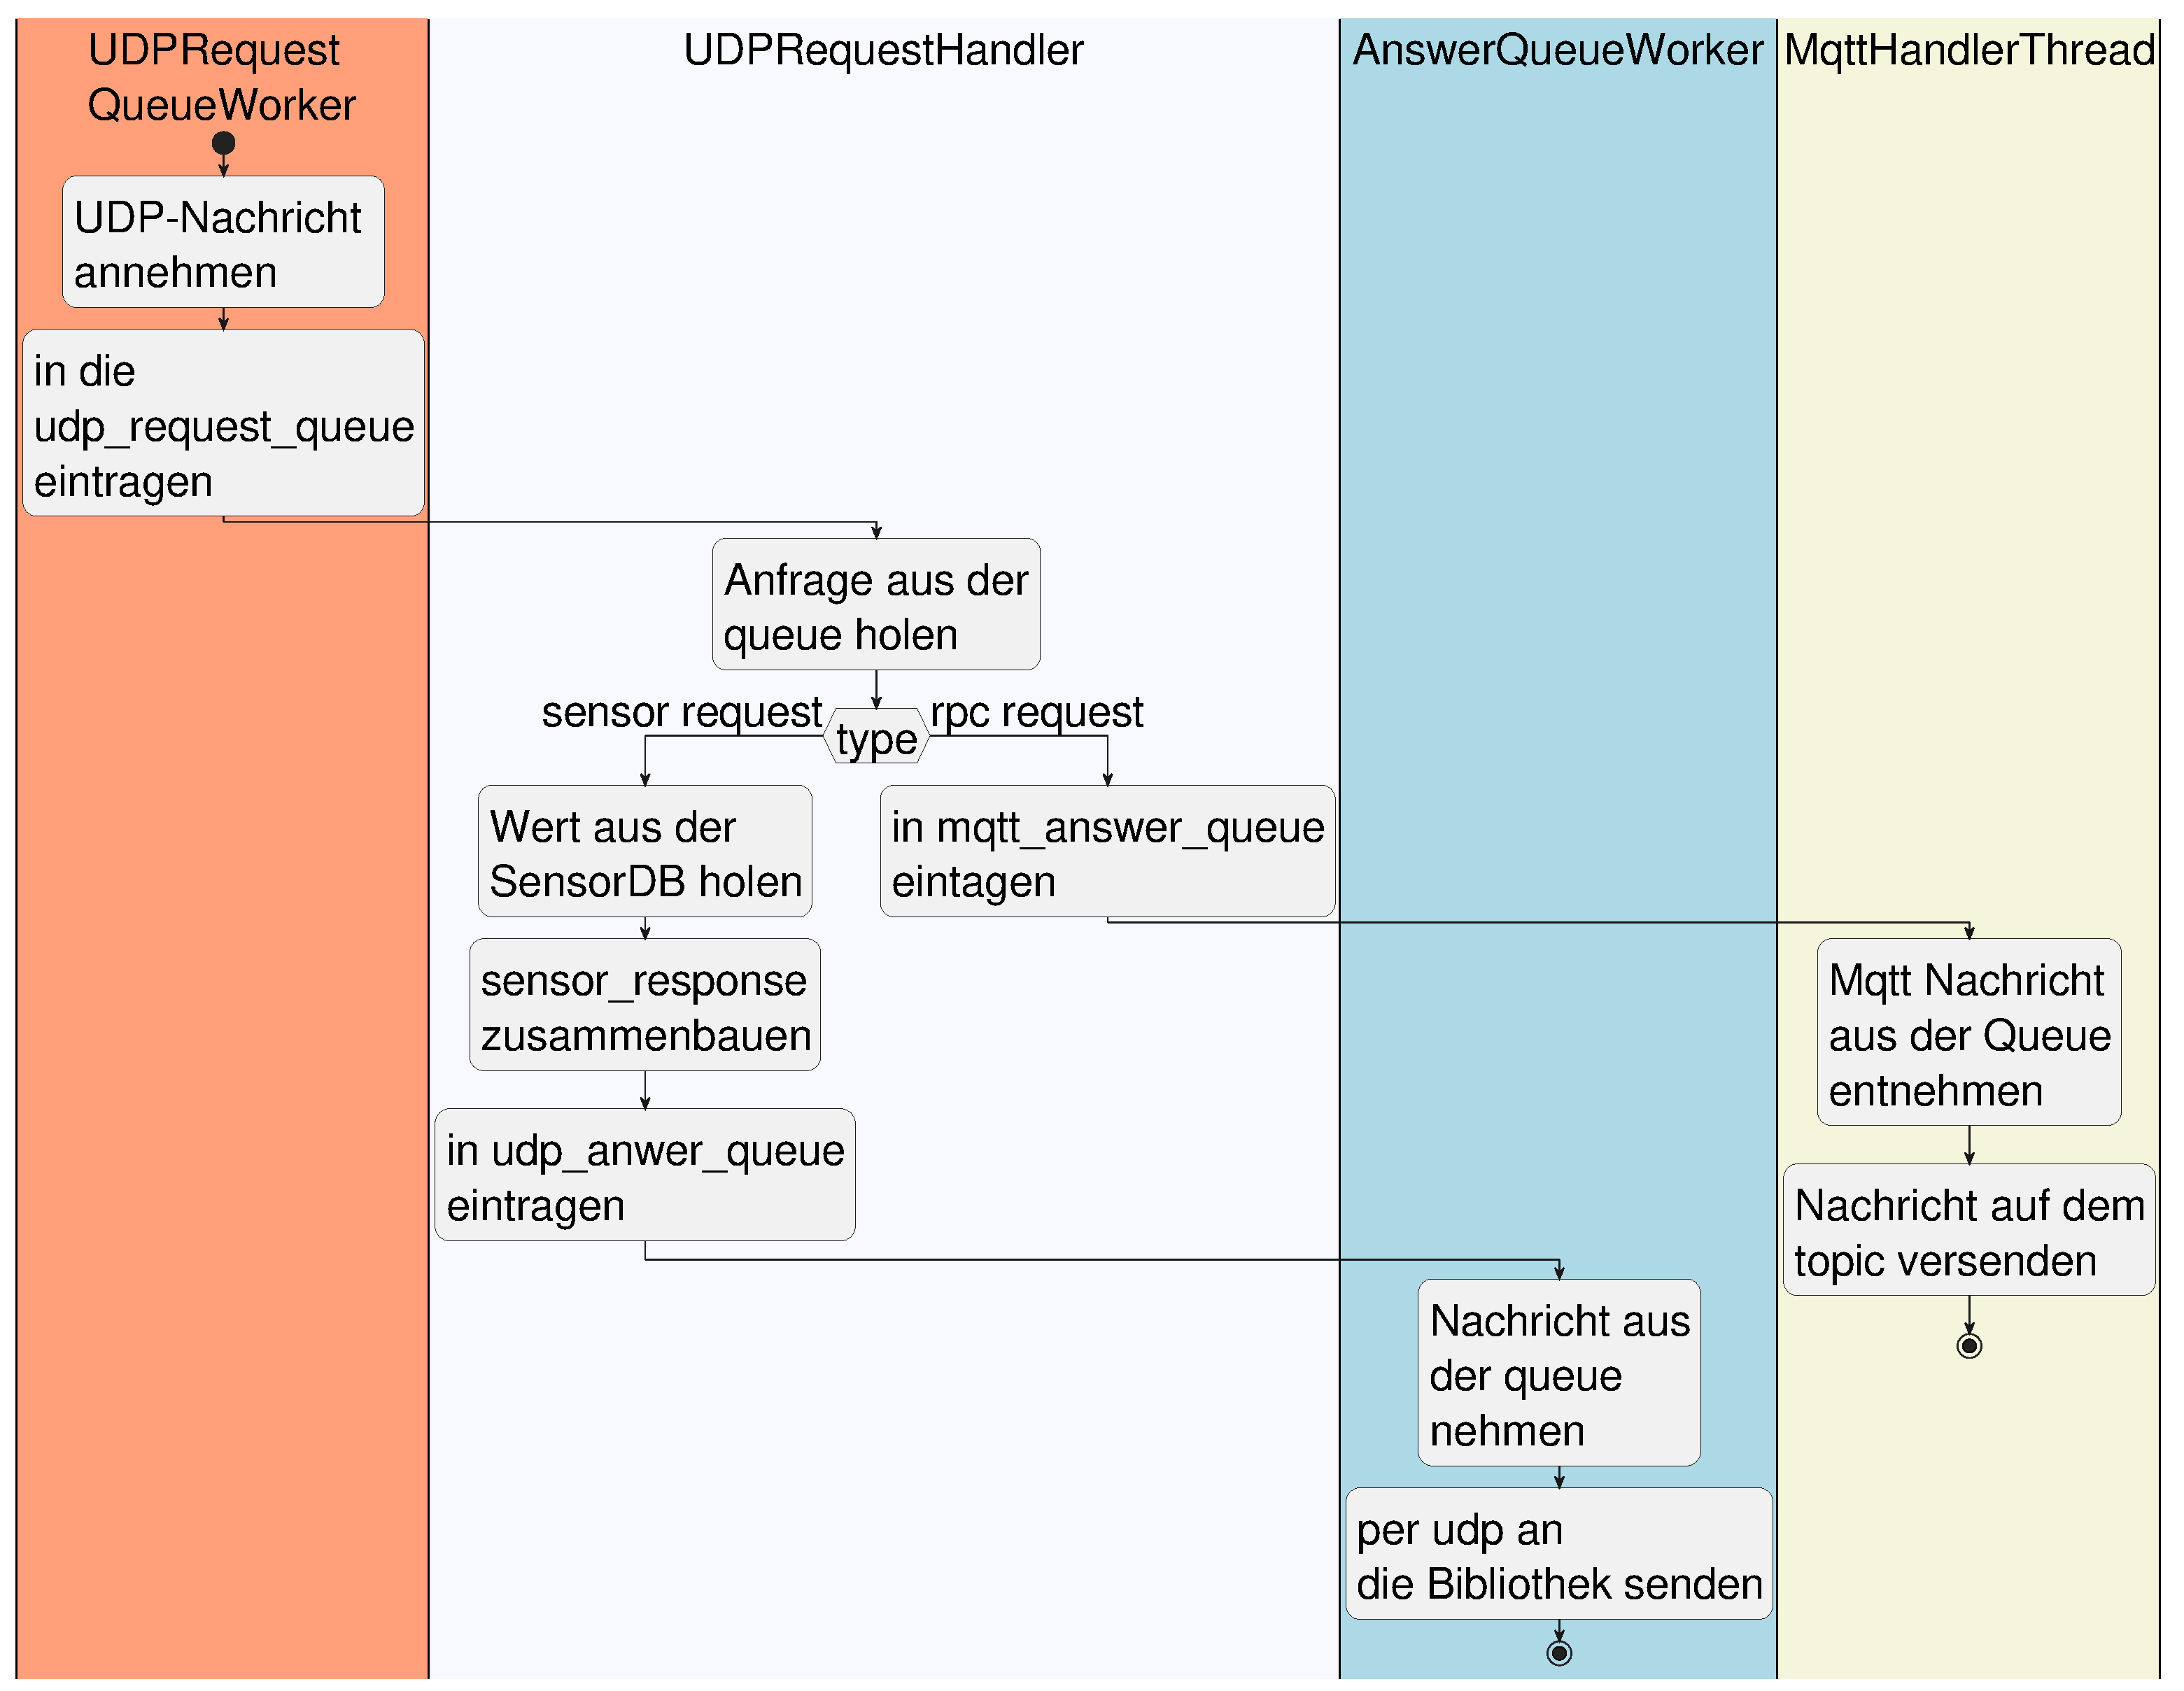
\includegraphics[width=\textwidth]{images/UDPRequestServerPath}
  \caption{Ablaufdiagramm UDP Request}
  \label{fig:serverUDPReqPath}
\end{figure}
Erreicht ein UDP Request den Server wird es vom UDPRequestQueue-Worker in eine UDP Request Queue gelegt.
Der UDPRequestHandler-Thread entnimmt die Nachricht und bestimmt den Anfragentyp.
Handelt es sich um eine Anfrage des Types RPC\_Request soll sie Aktionen auf dem Smartphone auslösen.
Sie muss an das Smartphone gesendet werden, was über MQTT möglich ist.
Dafür wird Sie ineine MqttAnswerQueue eingesetzt.
Der MQTTHandlerThread entnimmt Sie und sendet Sie per MQTT ab.
Ist Request hingegen ein SensorRequest, also eine Anfrage auf die ein Sensorwert geantwortet werden soll, wird der nachgefragte Sensorwert über die Klasse SensorDB entnommen und in die Udp\_answer\_queue eingetragen.
Der AnswerQueueWorker entnimmt die Anfrage und sendet Sie per udp an die Library zurück.

Zusammenfassend erfüllen die Komponenten folgende Aufgaben.
Der MQTTHandlerThread nimmt Nachrichten direkt per MQTT an und gibt die Anfrage weiter.
Außerdem sendet er Nachrichten per MQTT, falls welche anfallen.
Der MQTTRequestHandler kümmert sich um das Verfahren von MQTT Requests.
Der UDPRequestQueue Worker nimmt wie der MQTTHandlerThread Anfragen die per UDP übermittelt wurden an und gibt Sie zur Behandlung entsprechend weiter.
Er sendet jedoch im Gegensatz keine Responses zurück.
Hierfür gibt es den AnswerQueueWorker, dessen einzige Aufgabe es ist Antworten per UDP zurück zu übermitteln.

Die Kommunikation zwischen den Threads funktioniert über synchronisierte Queues des queue-Moduls\cite{python_queue} der cpython Implementierung.
Es handelt sich um eine threadsichere Monitorklasse, die einen gleichzeitigen Zugriff zweier unterschiedlicher Threads durch Locks verhindert.

\chapter{Programmierumgebung}\label{chap:libs}
Die Programmierumgebung ist die Schnittstelle, die die Programmierer für die Interaktion mit dem Smartphone in ihren Programmen verwenden.
Sie besteht aus einer Bibliothek, die Funktionen anbietet mit denen Programmierer Sensorwerte einlesen, oder Ausgaben auf dem Smartphone tätigen können.
Sie können die Funktionen in ihren bestehenden Quellcode einbinden und die Funktionen dort verwenden.
Die Bibliothek ist in den Programmiersprachen C, Java und Python vorhanden, damit Sie mit verschiedenen Programmiersprachen genutzt werden kann.
In Java und Python ist Sie zudem Plattformunabhängig.
Für C gibt es zwei Bibliotheken: Eine für Unix- und eine für Windows-Systeme.
In C ist die Bibliothek prozedural mit statischen Methoden, in Java und Python objektorientiert implementiert.

Werden die bereitgestellten Funktionen aufgerufen, werden standardisierte Anfragen im JSON-Format generiert und an die Kontrollanwendung gesendet.
Diese sendet die Daten gegebenenfalls an das Smartphone weiter oder antwortet direkt.
Eine Übersicht ist in Abbildung \ref{fig:Schnittstelle Bibliothek} dargestellt.
\begin{figure}[htbp]
  \centering
  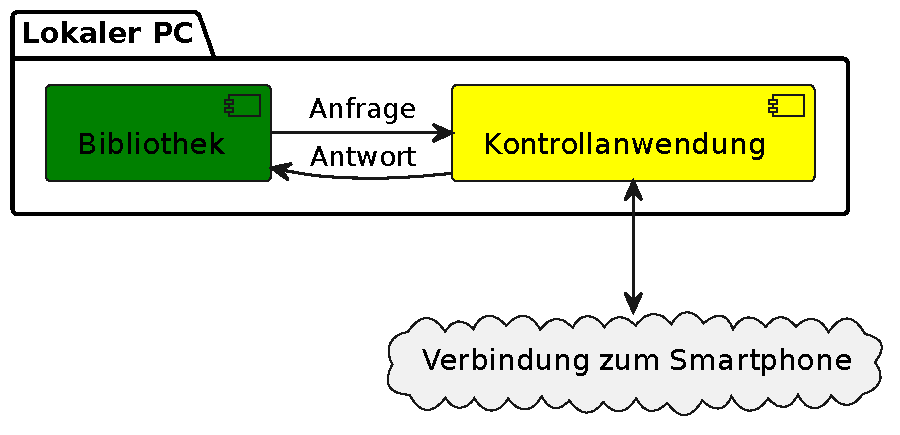
\includegraphics[width=.8\textwidth]{images/lib_server_connection}
  \caption{Schnittstellen der Bibliothek}
  \label{fig:Schnittstelle Bibliothek}
\end{figure}

Alle Anfragen werden über das UDP-Protokoll unter IPv4 versendet.
Das Kontrollprogramm ist auf dem Port 5006 erreichbar, Bibliotheken auf dem Port 5005.
Beide kommunizieren über die localhost-Adresse 127.0.0.1.
Dadurch werden Datagramme über das Loopback-Interface gesendet.
Das Loopback-Interface ist eine virtuelle Netzwerk-Schnittstelle des Betriebssystems eines PCs.
Pakete werden nicht über externe Netzwerk-Schnittstellen wie Netzwerkkarten versendet, sondern verbleiben im Netzwerk-Stack des Betriebssystems.
Die Latenzen sind dadurch mit weniger als 1 ms zur Verwendung der Lösung gering genug.
Zum Senden und Empfangen von Anfragen werden Sockets verwendet.
Für das Empfangen von Paketen müssen diese gebunden werden, für Sendevorgänge nicht.

Bei der Erstellung eines Phone-Objekts in Python und Java werden die Nachrichtenvorlagen für Anfragen und Antworten aus der Datei \texttt{protocol.json} geladen.
Die Datei muss sich im Dateisystem im gleichen Ordner befinden wie die Bibliothek.
Für die C-Bibliothek sind alle Methoden statisch definiert.
Es gibt somit keinen Start-Punkt zu dem die Datei \texttt{protocol.json} eingelesen werden kann.
Damit die Datei nicht für jeden Funktionsaufruf kontinuierlich eingelesen werden muss, muss Sie vom Programmierer einmal zum Start des Programms als cstring eingelesen werden.
Anschließend muss dieser cstring für jeden Aufruf einer Funktion der Bibliothek als Parameter angegeben werden.
Die Methode \texttt{get\_file\_content} kann, unter der Angabe des Dateipfades der \texttt{protocol.json}-Datei, aufgerufen werden um den Dateiinhalt einzulesen.
Zurückgegeben wird der Inhalt als cstring.
Diese Lösung verringert die Anzahl der Lesevorgänge und die damit verbundenen durch IO verursachten Latenzen.
Der Inhalt ist ab dem Einlesezeitpunkt auf dem Heap des Arbeitsspeichers gespeichert.
Der Programmierer muss diesen am Ende seines Programms durch den Aufruf der \texttt{free}-Funktion wieder freigeben.
%todo: klingt whack.
Die Ausgabe erscheint als direkter Grund der Annäherung.


\chapter{Evaluation}\label{chap:eval}
%todo: Messwerte stimmen noch nicht. Messung unter Vodaphone. Verzerrt. Check unter DSL.
%todo: auch gerne nochmal sprachlich drübergehen.
%todo: Intro fehlt. Worum geht's im Chapter? Qualitative und quantitative Bewertung.
In diesem Kapitel wird überprüft, ob die implementierte Lösung die Anforderungen erfüllt.
Überprüft wird die qualitive Nutzbarkeit der Lösung anhand der spezifizierten Anforderungen.
Für verschiedene Nutzungszenarien wie der Labor- oder Heimarbeit werden Latenzuverhalten gemessen.

In disem Kapitel wird die Verwendung des Frameworks anhand dem Beispiel \textit{Alarmanlage} vorgestellt.
\section{Verwendungsbeispiel}
Gezeigt wird, wie die Aufgabe in der Programmierumgebung gelöst wurde und wie sich die Aufgabe auf dem Smartphone äußert.
In der Programmierumgebung wird dabei die Python-Bibliothek verwendet.

Damit Nachrichten ausgetauscht werden können muss zuerst das Kontrollprogramm gestartet werden.
Es wird mit dem Befehl \texttt{python ./server.py} in einer lokalen Shell gestartet.
Der Vorgang wird in Abbildung \ref{fig:start_controll_app} dargestellt.
Es handelt sich um das Python-Skript \textit{server.py}.
\begin{figure}[htbp]
  \centering
  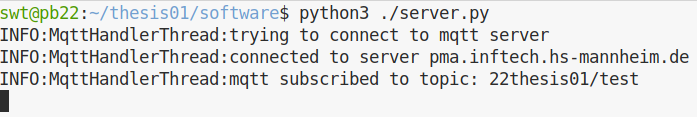
\includegraphics[width=.8\textwidth]{images/server_logging}
  \caption{Start der Kontrollanwendung}
  \label{fig:start_controll_app}
\end{figure}
Die Anwendung meldet, dass Sie sich erfolgreich mit dem MQTT-Broker verbunden und das korrekte Topic abboniert hat.
Die Kontrollanwendung loggt neben diesen Informationen auch rpc-requests und responses.
Sensor-requests und responses werden wegen ihrer hohen Anzahl nicht geloggt.

Die Implementierung der Lösung der Aufgabe ist in Listing \ref{lis:alarm} vorgestellt.

\lstset{language=python, captionpos=b, frame=single, numberstyle=\tiny, style=customcs}
\lstinputlisting[label=lis:alarm, caption=Alarmanlage-Beispiel]{listings/code_examples/alarm.py}
Die Bibliothek wird in Zeile 2 importiert.
Dafür muss die Datei \texttt{smartbit.py} im gleichen Ordner wie das Programm gespeichert sein.
In Zeile 4 wird ein Phone-Objekt erstellt, über das Sensor-Auslesemethoden wie \texttt{get\_x\_accel()} oder Smartphone-Ausgaben wie \texttt{vibrate()} augerufen werden können.
Da das Programm nie abbrechen soll, außer wenn es in der shell gestoppt wird, wird in einer While-True Schleife der Näherungssensor immer wieder abgefragt.
Anschließend wird eine halbe Sekunde gewartet um den Server nicht mit Anfragen zu überlasten.
Ist der abgerfragte Näherungssensorwert wie in der achten Zeile überprüft wird 0.0, dann liegt eine Näherung vor.
Auf dem Smartphone wird dann mit der  Methode \texttt{write\_text()} der Text ALARM usgegeben.
Das Smartphone vibriert 5 mal hintereinander im Abstand von 200 ms für eine Sekunde und lässt die Signal-LED blinken.
Insgesamt werden die RPC-Funktionen vibrate, toggle\_button und write\_text aufgerufen.
Keine dieser Funktionen liefert einen Rückgabewert.

Die Bibliothek sendet die Nachrichten an das Smartphone.
Nähert sich eine Person dem Smartphone wird der Code in der If-Bedingung ausgeführt.
Die jeweiligen Nachrichten werden als rpc\_request per UDP an die Kontrollanwendung gesendet.
Dort werden Sie angenommen, geloggt und per MQTT an das Smartphone weitergereicht.
Eine Übersicht der gesendeten Nachrichten ist in Abbildung \ref{fig:req_controll_app} zu sehen.
\begin{figure}[htbp]
  \centering
  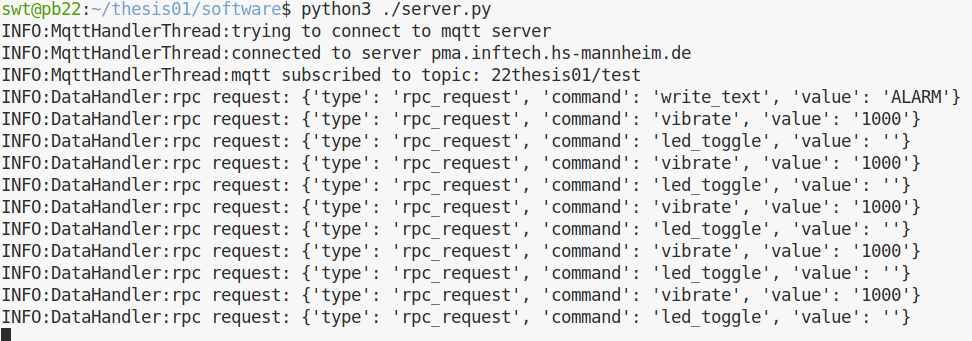
\includegraphics[width=\textwidth]{images/server_requests}
  \caption{Nachrichtenversand der Kontrollanwendung}
  \label{fig:req_controll_app}
\end{figure}
Die Nachrichten werden im JSON Format übertragen.
rpc\_requests haben ein Typ-Feld, ein Kommando und einen Paramterwert für das Kommando.
Write\_text ist für Textausgaben auf dem Smartphone, vibrate um das Smartphone vibrieren zu lassen und led\_toggle um die LED anzusprechen.
Für write\_text wird der gibt der Parameter-Wert den anzuzeigenden Text an.
Vibrate erwartet für value die Zeitdauer der vibrierung in ms.
led\_toggle erwartet keinen Parameterwert, da der gesamte Aufruf lediglich die Farbe der LED wechselt.
Es ist nicht vorgesehen, dass die Farbe manuell gesetzt werden kann.

Auf dem Smartphone ist die App zu Anfang im Initialmodus.
Dieser ist in Abbildung \ref{fig:initial_app} dargestellt.
\begin{figure}[htbp]
  \centering
  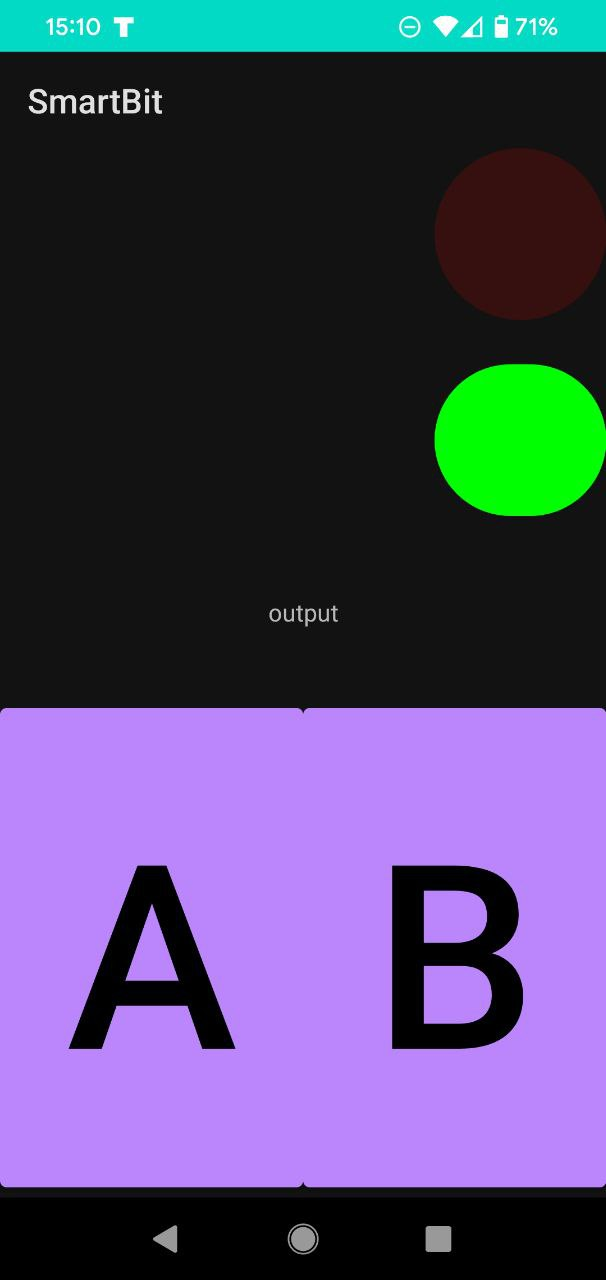
\includegraphics[height=0.4\textheight]{images/app_initial}
  \caption{Initialzustand der Anwendung}
  \label{fig:initial_app}
\end{figure}
Zu sehen sind zwei Buttons, beschriftet mit A und B.
Das textfeld liegt in der Mitte und zeigt zum Start den Text \textit{output} an.
Daneben gibt es noch eine Vorgangs-LED die ausgegraut oben rechts über der Signal-LED liegt.
Sie leuchtet, wenn gerade ein Vorgang wie das Ausführen einer Vibration auf dem Smartphone ausgeführt wird.

Nähert man sich dem Smartphone geht es über in den Alarmzustand der in Abbildung \ref{fig:app_alarm} dargestellt ist.
\begin{figure}[htbp]
  \centering
  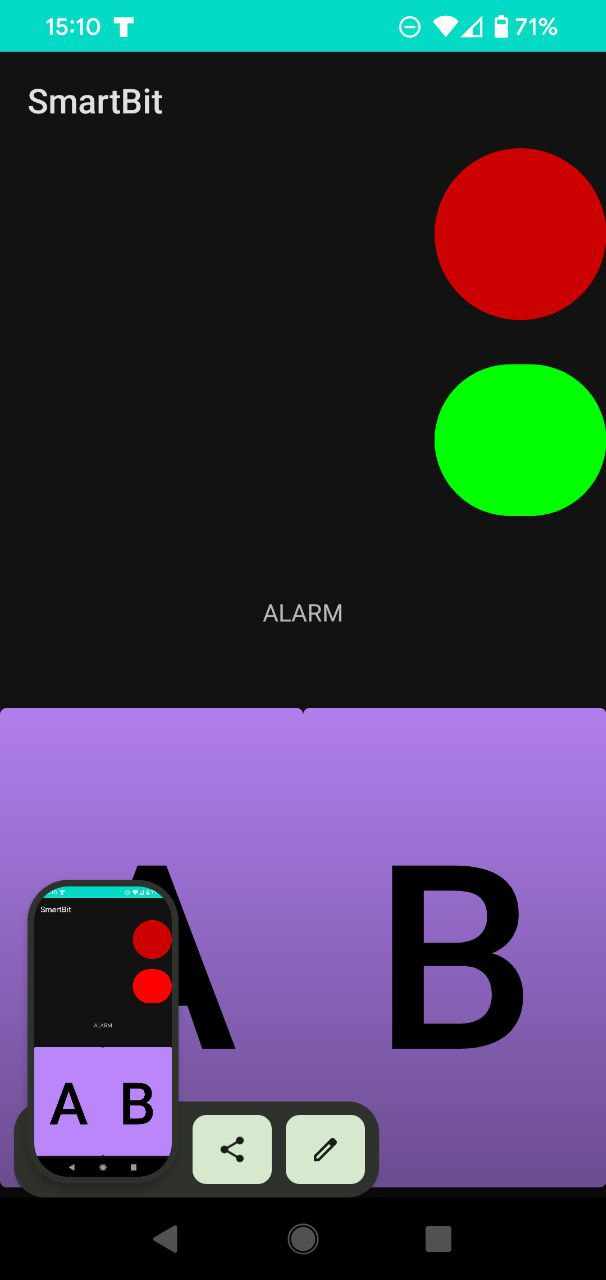
\includegraphics[height=0.4\textheight]{images/app_alarm}
  \caption{Initialzustand der Anwendung}
  \label{fig:app_alarm}
\end{figure}
Erkennbar ist, dass das Textfeld den Wert \textit{ALARM} darstellt.
Die Farbe der LED hat sich von grün auf rot und wieder auf grün geändert.
Das ist erkennbar an der kleinen Screenshot-Vorschau links unten die unmittelbar vor dem in der Abbildung zu sehenden Screenshot zu sehen ist.
Die Vorgangs-LED leuchtet rot um zu signalisieren dass gerade eine Ausgabe ausgeführt wird.
Nicht sichtbar ist das haptische vibrationsfeedback.
Hierfür dient jedoch die Vorgangs-LED.
Sie ist auch hilfreich um bei Smartphones mit sanften Vibrationsausgaben eine Ausgabe zu erkennen.
Die Reaktionszeit liegt unter einer Sekunde.

\section{Latenzmessung}
%todo: introsatz fehlt. liest sich unrund.

Transportwege müssen berücksichtigt werden.
Die Zeiten werden in drei verschiedenen Umgebungen überprüft: In nächster Nähe zum MQTT-Server, in mittlerer Nähe und in einer virtuellen Umgebung über ein simuliertes NAT-Netzwerk.

Damit die Benutzbarkeit sichergestellt ist, müssen Latenzzeiten zwischen Smartphone und Programmierumgebung in einem akzeptablen Rahmen liegen.
Um dies herauszufinden werden die Latenzzeiten gemessen.
In diesem Kapitel wird die Latenzzeit von drei Standorten aus gemessen.

Der erste Einsatzort ist im gleichen Netzbereich wie der MQTT-Broker wodurch die Transferstrecke reduziert wird.
Neben der Latenzzeit zum Broker ist jedoch auch die Anzahl der angemeldeten Geräte am gleichen AccessPoint interessant.
Da die Geräte in direktem Wettbewerb um Sendezeit stehen bedeuten mehr Geräte an einem AccessPoint größere Latenzen.
In den Messungen werden nur WLAN-Verbindungen nach dem Standard WLAN 802.11n berücksichtigt.
Es sind dabei stets beide Geräte, Lokaler PC und Smartphone per WLAN mit dem Internet verbunden.
Untersucht wird lediglich die Zeitspanne zwischen rpc\_request und rpc\_response.
Sensor\_requests kommunizieren stets per loopback-interface mit der Kontrollanwendung.
Daher die Latenzzeiten gering.
Im Durchschnitt belaufen Sie sich auf unter 1ms.
Die Messungen sind  für den Fall interessant, für den Studierende an der Hochschule die Lösung nutzen möchten.
Zum Beispiel in Laboren.

Der zweite Einsatzort ist ein Heimnetz, das etwa 8 Hops entfernt vom MQTT-Broker liegt.
Etwa 8 Geräte sind dabei auf dem Access Point angemeldet.
Die Messergebnisse sind relevant für die Heimarbeit oder das Erledigen von Hausaufgaben.
Die Ergebnisse sind in Abbildung \ref{fig:measure_home} dargestellt.
\begin{figure}[htbp]
  \centering
  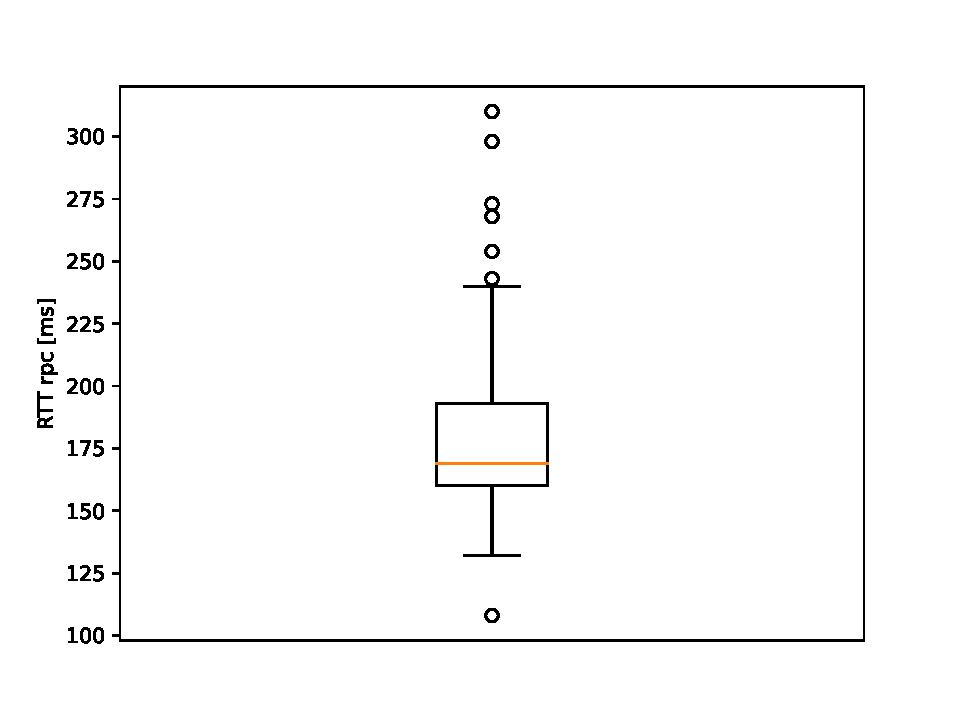
\includegraphics[width=0.6\textwidth]{images/timing_at_home}
  \caption{Zeitmessungen im Heimnetz}
  \label{fig:measure_home}
\end{figure}
Insgesamt wurden 100 Messungen durchgeführt.
Im Mittel beträgt die Reaktionszeit 537 ms.
Die Streuung ist bei einer Standardabweichung von 238ms allerdings auch sehr breit gestreut.
Alle Messungen blieben jedoch unter 1s Reaktionszeit.

Der letzte Einsatzort ist in einer virtuellen Maschine auf dem lokalen PC das über den virtuellen Netzwerkkontroller aus einem NAT-Netzbereich auf das Internet zugreift.
Das Smartphone befindet sich direkt im Netzbereich des lokalen PCs.
Die gemessenen Daten sind in Abbildung \ref{fig:measure_vm} dargestellt.
\begin{figure}[htbp]
  \centering
  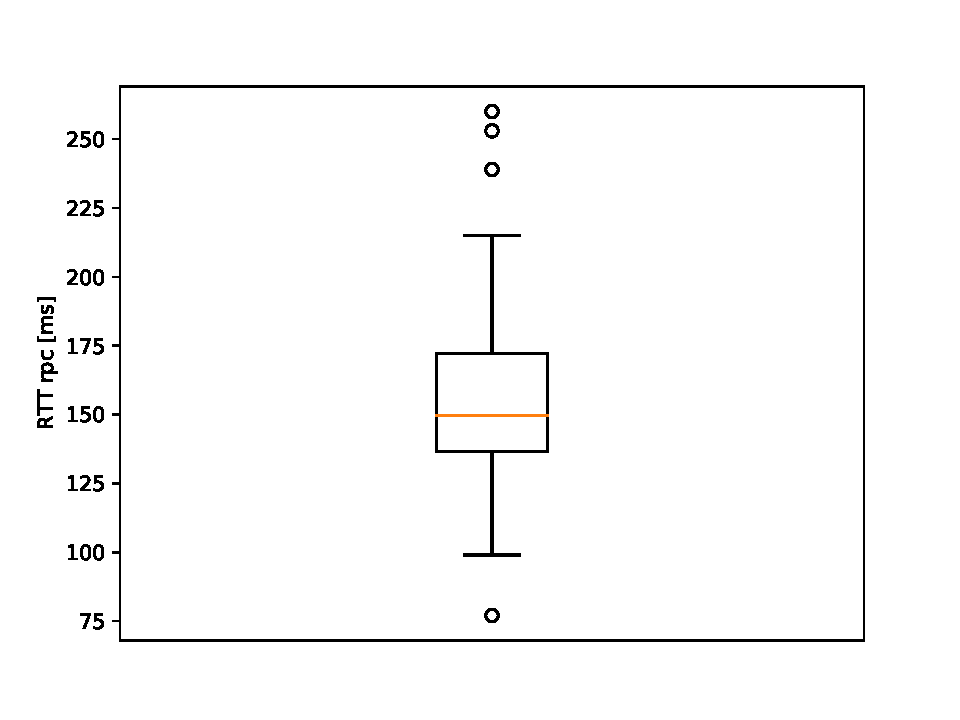
\includegraphics[width=0.6\textwidth]{images/timing_vm}
  \caption{Zeitmessungen in der virtuellen Maschine}
  \label{fig:measure_vm}
\end{figure}
Wieder wurden 100 Messungen vorgenommen.
Im Mittel beträgt die Reaktionszeit nun 3255 ms.
Die Streuung ist mit einer Standardabweichung von 845 ms relativ gleichgroß.
Die Reaktionszeit ist also im Durchschnitt sehr hoch, etwa sechs mal langsamer als bei einer Verwendung der Programmierumgebung auf dem Hostsystem.
Eine direkte Assoziation zwischen Eingabe und Ausgabe kann nicht garantiert werden.

Latenzprobleme per MQTT treten nicht auf.
Trotz einem QOS-Level 0 werden auch Ausgabeanfragen sicher übertragen und ausgeführt.
Da die Nachrichten über TLS übertragen werden ist der Austausch sicher.
Logging-Möglichkeiten in der Kontrollanwendung und der Android-App erleichterten die Entwicklung sehr und halfen bei der Fehlersuche.

\chapter{Fazit}\label{chap:fazit}
Die implementierte Lösung erfüllt die Anforderungen zufriedenstellend.
Die im Vorfeld durchgeführte Konzeption der Lösung ermöglichte eine problemlose Implementierung.
Während der Entwicklung wurden jedoch einige Designentscheidungen getroffen, welche die Lösung beschränken.
Sensordaten werden von der Kontrollanwendung nicht für einzelne Geräte eingespeichert.
Es ist nicht möglich Programmcode simultan auf mehreren Smartphones gleichzeitig auszuführen.
Gruppen-Sessions können nicht erstellt werden.
Für Programme die die Java und Python-Schnittstelle könnte dies unintuitiv erscheinen.
Die Bedeutung eines Phone-Objektes lässt auf eine zwischen Einzelgeräten unterscheidende Verwendung schließen.
Ein weiterer Nachteil der Benutzerfreundlichkeit besteht in der zwingenden Verwendung von Hilfs-Bibliotheken für den Nachrichtenaustausch über JSON.
Sowohl für Java, als auch für C sind zusätzliche JSON-Parser für die Kommunikation zwischen Bibliothek und Kontrollanwendung nötig.
Für eine erfolgreiche Kompilierung in C muss der Dateipfad für diesen dem Linker bekannt gemacht werden.
Für die interne Struktur ist die Datenverwaltung innerhalb des Programms ausreichend.
Durch den asynchronen Ansatz des Multithreading können beide Kommunikationspartner gleichzeitig über das Kontrollprogramm kommunizieren und zwischengespeicherte Daten auslesen oder bearbeiten.
Die Möglichkeit mehrere Werte zum internen Datenspeicher hinzuzufügen wird jedoch nicht unterstützt.
Häufige Sensor-Anfragen werden mit dem gleichen, einzeln zwischengespeicherten Sensorwert beantwortet, welcher zusätzlich kein Ablaufdatum besitzt.
Abbrüche der Übertragung resultieren in der kontinuierlichen Übermittlung des zuletzt eingespeicherten Sensorwerts.

Zur Ablösung von Hilfsbibliotheken eignet sich die Verwendung eines Binärprotokolls.
In Enumerationen konvertierte Nachrichtenformate und Parameter könnten statt der implementierten Darstellung mit JSON eingesetzt werden.
Dadurch entfiehle nicht nur der Nachteil der unintuitiven Einbindung.
Die Nachrichtengröße würde ebenfalls verringert werden.
Energieeffizienz der Android-App wurde zum Vorteil der Latenzreduzierung während der Implementierung nicht wesentlich berücksichtigt.
Zum Start der Anwendung werden die Sensormessprozesse unmittelbar gestartet und Sensorwerte an die Kontrollanwendung gesendet, was einen erhöhten Energieverbrauch bedeutet.
Sollten sich die Startzeiten der Sensormessprozesse nicht wesentlich auf die Latenzen auswirken, wäre eine auf Anfragen basierende Sensmessdatenübertragung erwägenswert um den Energieverbrauch zu reduzieren.

% Listen wenn überhaupt ans Ende und nicht an den Anfang.
% Meist ist das aber unnötig.
% List of abbrev
\listoffigures % Liste der Abbildungen 
\listoftables % Liste der Tabellen
\printglossary[type=\acronymtype, title={Abkürzungsverzeichnis}]

\newpage

%check: hat das hier geklappt?


\bibliographystyle{plain} % Literaturverzeichnis
\begin{btSect}{thesis} % mit bibtopic Quellen trennen
\addcontentsline{toc}{chapter}{Literaturverzeichnis und Online-Quellen}
\section*{Literaturverzeichnis}
\btPrintCited
\end{btSect}
\begin{btSect}{online}
\section*{Online-Quellen}
\btPrintCited
%\bibliography{online}
\end{btSect}
% dann mit "bibtex thesis1" und "bibtex thesis2" arbeiten

\end{document}
;;; Local Variables:
;;; ispell-local-dictionary: "de_DE-neu"
;;; End:


